% Options for packages loaded elsewhere
\PassOptionsToPackage{unicode}{hyperref}
\PassOptionsToPackage{hyphens}{url}
%
\documentclass[
]{book}
\usepackage{amsmath,amssymb}
\usepackage{lmodern}
\usepackage{ifxetex,ifluatex}
\ifnum 0\ifxetex 1\fi\ifluatex 1\fi=0 % if pdftex
  \usepackage[T1]{fontenc}
  \usepackage[utf8]{inputenc}
  \usepackage{textcomp} % provide euro and other symbols
\else % if luatex or xetex
  \usepackage{unicode-math}
  \defaultfontfeatures{Scale=MatchLowercase}
  \defaultfontfeatures[\rmfamily]{Ligatures=TeX,Scale=1}
\fi
% Use upquote if available, for straight quotes in verbatim environments
\IfFileExists{upquote.sty}{\usepackage{upquote}}{}
\IfFileExists{microtype.sty}{% use microtype if available
  \usepackage[]{microtype}
  \UseMicrotypeSet[protrusion]{basicmath} % disable protrusion for tt fonts
}{}
\makeatletter
\@ifundefined{KOMAClassName}{% if non-KOMA class
  \IfFileExists{parskip.sty}{%
    \usepackage{parskip}
  }{% else
    \setlength{\parindent}{0pt}
    \setlength{\parskip}{6pt plus 2pt minus 1pt}}
}{% if KOMA class
  \KOMAoptions{parskip=half}}
\makeatother
\usepackage{xcolor}
\IfFileExists{xurl.sty}{\usepackage{xurl}}{} % add URL line breaks if available
\IfFileExists{bookmark.sty}{\usepackage{bookmark}}{\usepackage{hyperref}}
\hypersetup{
  pdftitle={Toolbox},
  pdfauthor={Bhaswar Chakma},
  hidelinks,
  pdfcreator={LaTeX via pandoc}}
\urlstyle{same} % disable monospaced font for URLs
\usepackage{color}
\usepackage{fancyvrb}
\newcommand{\VerbBar}{|}
\newcommand{\VERB}{\Verb[commandchars=\\\{\}]}
\DefineVerbatimEnvironment{Highlighting}{Verbatim}{commandchars=\\\{\}}
% Add ',fontsize=\small' for more characters per line
\usepackage{framed}
\definecolor{shadecolor}{RGB}{248,248,248}
\newenvironment{Shaded}{\begin{snugshade}}{\end{snugshade}}
\newcommand{\AlertTok}[1]{\textcolor[rgb]{0.94,0.16,0.16}{#1}}
\newcommand{\AnnotationTok}[1]{\textcolor[rgb]{0.56,0.35,0.01}{\textbf{\textit{#1}}}}
\newcommand{\AttributeTok}[1]{\textcolor[rgb]{0.77,0.63,0.00}{#1}}
\newcommand{\BaseNTok}[1]{\textcolor[rgb]{0.00,0.00,0.81}{#1}}
\newcommand{\BuiltInTok}[1]{#1}
\newcommand{\CharTok}[1]{\textcolor[rgb]{0.31,0.60,0.02}{#1}}
\newcommand{\CommentTok}[1]{\textcolor[rgb]{0.56,0.35,0.01}{\textit{#1}}}
\newcommand{\CommentVarTok}[1]{\textcolor[rgb]{0.56,0.35,0.01}{\textbf{\textit{#1}}}}
\newcommand{\ConstantTok}[1]{\textcolor[rgb]{0.00,0.00,0.00}{#1}}
\newcommand{\ControlFlowTok}[1]{\textcolor[rgb]{0.13,0.29,0.53}{\textbf{#1}}}
\newcommand{\DataTypeTok}[1]{\textcolor[rgb]{0.13,0.29,0.53}{#1}}
\newcommand{\DecValTok}[1]{\textcolor[rgb]{0.00,0.00,0.81}{#1}}
\newcommand{\DocumentationTok}[1]{\textcolor[rgb]{0.56,0.35,0.01}{\textbf{\textit{#1}}}}
\newcommand{\ErrorTok}[1]{\textcolor[rgb]{0.64,0.00,0.00}{\textbf{#1}}}
\newcommand{\ExtensionTok}[1]{#1}
\newcommand{\FloatTok}[1]{\textcolor[rgb]{0.00,0.00,0.81}{#1}}
\newcommand{\FunctionTok}[1]{\textcolor[rgb]{0.00,0.00,0.00}{#1}}
\newcommand{\ImportTok}[1]{#1}
\newcommand{\InformationTok}[1]{\textcolor[rgb]{0.56,0.35,0.01}{\textbf{\textit{#1}}}}
\newcommand{\KeywordTok}[1]{\textcolor[rgb]{0.13,0.29,0.53}{\textbf{#1}}}
\newcommand{\NormalTok}[1]{#1}
\newcommand{\OperatorTok}[1]{\textcolor[rgb]{0.81,0.36,0.00}{\textbf{#1}}}
\newcommand{\OtherTok}[1]{\textcolor[rgb]{0.56,0.35,0.01}{#1}}
\newcommand{\PreprocessorTok}[1]{\textcolor[rgb]{0.56,0.35,0.01}{\textit{#1}}}
\newcommand{\RegionMarkerTok}[1]{#1}
\newcommand{\SpecialCharTok}[1]{\textcolor[rgb]{0.00,0.00,0.00}{#1}}
\newcommand{\SpecialStringTok}[1]{\textcolor[rgb]{0.31,0.60,0.02}{#1}}
\newcommand{\StringTok}[1]{\textcolor[rgb]{0.31,0.60,0.02}{#1}}
\newcommand{\VariableTok}[1]{\textcolor[rgb]{0.00,0.00,0.00}{#1}}
\newcommand{\VerbatimStringTok}[1]{\textcolor[rgb]{0.31,0.60,0.02}{#1}}
\newcommand{\WarningTok}[1]{\textcolor[rgb]{0.56,0.35,0.01}{\textbf{\textit{#1}}}}
\usepackage{longtable,booktabs,array}
\usepackage{calc} % for calculating minipage widths
% Correct order of tables after \paragraph or \subparagraph
\usepackage{etoolbox}
\makeatletter
\patchcmd\longtable{\par}{\if@noskipsec\mbox{}\fi\par}{}{}
\makeatother
% Allow footnotes in longtable head/foot
\IfFileExists{footnotehyper.sty}{\usepackage{footnotehyper}}{\usepackage{footnote}}
\makesavenoteenv{longtable}
\usepackage{graphicx}
\makeatletter
\def\maxwidth{\ifdim\Gin@nat@width>\linewidth\linewidth\else\Gin@nat@width\fi}
\def\maxheight{\ifdim\Gin@nat@height>\textheight\textheight\else\Gin@nat@height\fi}
\makeatother
% Scale images if necessary, so that they will not overflow the page
% margins by default, and it is still possible to overwrite the defaults
% using explicit options in \includegraphics[width, height, ...]{}
\setkeys{Gin}{width=\maxwidth,height=\maxheight,keepaspectratio}
% Set default figure placement to htbp
\makeatletter
\def\fps@figure{htbp}
\makeatother
\setlength{\emergencystretch}{3em} % prevent overfull lines
\providecommand{\tightlist}{%
  \setlength{\itemsep}{0pt}\setlength{\parskip}{0pt}}
\setcounter{secnumdepth}{5}
\usepackage{booktabs}
\usepackage{amsthm}
\makeatletter
\def\thm@space@setup{%
  \thm@preskip=8pt plus 2pt minus 4pt
  \thm@postskip=\thm@preskip
}
\makeatother
\ifluatex
  \usepackage{selnolig}  % disable illegal ligatures
\fi
\usepackage[]{natbib}
\bibliographystyle{apalike}

\title{Toolbox}
\author{Bhaswar Chakma}
\date{2021-08-20}

\begin{document}
\maketitle

{
\setcounter{tocdepth}{1}
\tableofcontents
}
\hypertarget{section}{%
\chapter*{}\label{section}}
\addcontentsline{toc}{chapter}{}

\hypertarget{dplyr-vs-pandas-numpy}{%
\chapter{dplyr vs pandas \& numpy}\label{dplyr-vs-pandas-numpy}}

We will use the five \href{https://dplyr.tidyverse.org/}{dplyr verbs} (also \href{https://pandas.pydata.org/pandas-docs/stable/getting_started/comparison/comparison_with_r.html}{pandas' guide}) for comparison

\begin{itemize}
\item
  \texttt{select()} picks variables based on their names.
\item
  \texttt{mutate()} adds new variables that are functions of existing variables
\item
  \texttt{filter()} picks cases based on their values.
\item
  \texttt{summarise()} reduces multiple values down to a single summary.
\item
  \texttt{arrange()} changes the ordering of the rows.
\end{itemize}

and use the following toy data to apply the verbs.

\begin{longtable}[]{@{}llr@{}}
\toprule
name & gender & grade \\
\midrule
\endhead
Barney & Male & 10 \\
Ted & Male & 11 \\
Marshall & Male & 13 \\
Lilly & Female & 12 \\
Robin & Female & 14 \\
\bottomrule
\end{longtable}

{\textbf{Create Toy Data}}

dplyr

pandas

\begin{Shaded}
\begin{Highlighting}[]
\NormalTok{df }\OtherTok{\textless{}{-}} \FunctionTok{tibble}\NormalTok{(}
  \AttributeTok{name =} \FunctionTok{c}\NormalTok{(}\StringTok{"Barney"}\NormalTok{, }\StringTok{"Ted"}\NormalTok{, }\StringTok{"Marshall"}\NormalTok{,}
           \StringTok{"Lilly"}\NormalTok{,}\StringTok{"Robin"}\NormalTok{),}
  \AttributeTok{gender =} \FunctionTok{c}\NormalTok{(}\StringTok{"Male"}\NormalTok{, }\StringTok{"Male"}\NormalTok{,}\StringTok{"Male"}\NormalTok{,}
             \StringTok{"Female"}\NormalTok{, }\StringTok{"Female"}\NormalTok{),}
  \AttributeTok{grade =} \FunctionTok{c}\NormalTok{(}\DecValTok{10}\NormalTok{, }\DecValTok{11}\NormalTok{, }\DecValTok{13}\NormalTok{, }\DecValTok{12}\NormalTok{, }\DecValTok{14}\NormalTok{)}
\NormalTok{)}
\NormalTok{df}
\end{Highlighting}
\end{Shaded}

\begin{verbatim}
## # A tibble: 5 x 3
##   name     gender grade
##   <chr>    <chr>  <dbl>
## 1 Barney   Male      10
## 2 Ted      Male      11
## 3 Marshall Male      13
## 4 Lilly    Female    12
## 5 Robin    Female    14
\end{verbatim}

\begin{Shaded}
\begin{Highlighting}[]
\NormalTok{df }\OperatorTok{=}\NormalTok{ pd.DataFrame(\{}
  \StringTok{\textquotesingle{}name\textquotesingle{}}\NormalTok{:[}\StringTok{"Barney"}\NormalTok{, }\StringTok{"Ted"}\NormalTok{, }\StringTok{"Marshall"}\NormalTok{,}
          \StringTok{"Lilly"}\NormalTok{, }\StringTok{"Robin"}\NormalTok{],}
  \StringTok{\textquotesingle{}gender\textquotesingle{}}\NormalTok{:[}\StringTok{"Male"}\NormalTok{, }\StringTok{"Male"}\NormalTok{,}\StringTok{"Male"}\NormalTok{, }
            \StringTok{"Female"}\NormalTok{, }\StringTok{"Female"}\NormalTok{],}
  \StringTok{\textquotesingle{}grade\textquotesingle{}}\NormalTok{:[}\DecValTok{10}\NormalTok{, }\DecValTok{11}\NormalTok{, }\DecValTok{13}\NormalTok{, }\DecValTok{12}\NormalTok{, }\DecValTok{14}\NormalTok{] }
\NormalTok{\})}
\NormalTok{df}
\end{Highlighting}
\end{Shaded}

\begin{verbatim}
##        name  gender  grade
## 0    Barney    Male     10
## 1       Ted    Male     11
## 2  Marshall    Male     13
## 3     Lilly  Female     12
## 4     Robin  Female     14
\end{verbatim}

{\textbf{Check Data Structure}}

dplyr

pandas

\begin{Shaded}
\begin{Highlighting}[]
\FunctionTok{glimpse}\NormalTok{(df)}
\end{Highlighting}
\end{Shaded}

\begin{verbatim}
## Rows: 5
## Columns: 3
## $ name   <chr> "Barney", "Ted", "Marshall", "Lilly", "Robin"
## $ gender <chr> "Male", "Male", "Male", "Female", "Female"
## $ grade  <dbl> 10, 11, 13, 12, 14
\end{verbatim}

\begin{Shaded}
\begin{Highlighting}[]
\NormalTok{df.dtypes}
\end{Highlighting}
\end{Shaded}

\begin{verbatim}
## name      object
## gender    object
## grade      int64
## dtype: object
\end{verbatim}

\begin{Shaded}
\begin{Highlighting}[]
\NormalTok{df.shape}
\end{Highlighting}
\end{Shaded}

\begin{verbatim}
## (5, 3)
\end{verbatim}

\begin{Shaded}
\begin{Highlighting}[]
\NormalTok{df.info()}
\end{Highlighting}
\end{Shaded}

\begin{verbatim}
## <class 'pandas.core.frame.DataFrame'>
## RangeIndex: 5 entries, 0 to 4
## Data columns (total 3 columns):
## name      5 non-null object
## gender    5 non-null object
## grade     5 non-null int64
## dtypes: int64(1), object(2)
## memory usage: 248.0+ bytes
\end{verbatim}

\hypertarget{select}{%
\section{\texorpdfstring{\texttt{select()}}{select()}}\label{select}}

{\textbf{Task: Pick the variables \texttt{name} and \texttt{grade}.
}}

dplyr

pandas

\begin{Shaded}
\begin{Highlighting}[]
\NormalTok{df }\SpecialCharTok{\%\textgreater{}\%} 
  \FunctionTok{select}\NormalTok{(name, grade)}
\end{Highlighting}
\end{Shaded}

\begin{verbatim}
## # A tibble: 5 x 2
##   name     grade
##   <chr>    <dbl>
## 1 Barney      10
## 2 Ted         11
## 3 Marshall    13
## 4 Lilly       12
## 5 Robin       14
\end{verbatim}

\begin{Shaded}
\begin{Highlighting}[]
\NormalTok{df[[}\StringTok{\textquotesingle{}name\textquotesingle{}}\NormalTok{, }\StringTok{\textquotesingle{}grade\textquotesingle{}}\NormalTok{]]}
\end{Highlighting}
\end{Shaded}

\begin{verbatim}
##        name  grade
## 0    Barney     10
## 1       Ted     11
## 2  Marshall     13
## 3     Lilly     12
## 4     Robin     14
\end{verbatim}

\begin{Shaded}
\begin{Highlighting}[]
\CommentTok{\# or}
\NormalTok{df.drop(columns }\OperatorTok{=}\NormalTok{ [}\StringTok{\textquotesingle{}gender\textquotesingle{}}\NormalTok{])}
\end{Highlighting}
\end{Shaded}

\begin{verbatim}
##        name  grade
## 0    Barney     10
## 1       Ted     11
## 2  Marshall     13
## 3     Lilly     12
## 4     Robin     14
\end{verbatim}

\begin{Shaded}
\begin{Highlighting}[]
\CommentTok{\# or}
\NormalTok{df.drop([}\StringTok{\textquotesingle{}gender\textquotesingle{}}\NormalTok{], axis }\OperatorTok{=} \DecValTok{1}\NormalTok{)}
\end{Highlighting}
\end{Shaded}

\begin{verbatim}
##        name  grade
## 0    Barney     10
## 1       Ted     11
## 2  Marshall     13
## 3     Lilly     12
## 4     Robin     14
\end{verbatim}

\textbf{Using positions of columns:}

\begin{Shaded}
\begin{Highlighting}[]
\NormalTok{df[df.columns[[}\DecValTok{0}\NormalTok{,}\DecValTok{2}\NormalTok{]]]}
\end{Highlighting}
\end{Shaded}

\begin{verbatim}
##        name  grade
## 0    Barney     10
## 1       Ted     11
## 2  Marshall     13
## 3     Lilly     12
## 4     Robin     14
\end{verbatim}

\begin{Shaded}
\begin{Highlighting}[]
\NormalTok{df.iloc[:, [}\DecValTok{0}\NormalTok{,}\DecValTok{2}\NormalTok{]]}
\end{Highlighting}
\end{Shaded}

\begin{verbatim}
##        name  grade
## 0    Barney     10
## 1       Ted     11
## 2  Marshall     13
## 3     Lilly     12
## 4     Robin     14
\end{verbatim}

\hypertarget{mutate}{%
\section{\texorpdfstring{\texttt{mutate()}}{mutate()}}\label{mutate}}

{\textbf{Task: Generate a variable \texttt{grade\_p}, expressing grade out of 100.
}}

dplyr

pandas

\begin{Shaded}
\begin{Highlighting}[]
\NormalTok{df }\SpecialCharTok{\%\textgreater{}\%} 
  \FunctionTok{mutate}\NormalTok{(}\AttributeTok{grade\_p =}\NormalTok{ grade}\SpecialCharTok{/}\DecValTok{20}\SpecialCharTok{*}\DecValTok{100}\NormalTok{)}
\end{Highlighting}
\end{Shaded}

\begin{verbatim}
## # A tibble: 5 x 4
##   name     gender grade grade_p
##   <chr>    <chr>  <dbl>   <dbl>
## 1 Barney   Male      10      50
## 2 Ted      Male      11      55
## 3 Marshall Male      13      65
## 4 Lilly    Female    12      60
## 5 Robin    Female    14      70
\end{verbatim}

\begin{Shaded}
\begin{Highlighting}[]
\NormalTok{df[}\StringTok{\textquotesingle{}grade\_p\textquotesingle{}}\NormalTok{] }\OperatorTok{=}\NormalTok{ df[}\StringTok{\textquotesingle{}grade\textquotesingle{}}\NormalTok{]}\OperatorTok{/}\DecValTok{20}\OperatorTok{*}\DecValTok{100}
\NormalTok{df}
\end{Highlighting}
\end{Shaded}

\begin{verbatim}
##        name  gender  grade  grade_p
## 0    Barney    Male     10     50.0
## 1       Ted    Male     11     55.0
## 2  Marshall    Male     13     65.0
## 3     Lilly  Female     12     60.0
## 4     Robin  Female     14     70.0
\end{verbatim}

\begin{Shaded}
\begin{Highlighting}[]
\CommentTok{\# now drop the newly created variable}
\NormalTok{df.drop(columns }\OperatorTok{=} \StringTok{\textquotesingle{}grade\_p\textquotesingle{}}\NormalTok{, inplace }\OperatorTok{=} \VariableTok{True}\NormalTok{)}
\end{Highlighting}
\end{Shaded}

\hypertarget{filter}{%
\section{\texorpdfstring{\texttt{filter()}}{filter()}}\label{filter}}

{\textbf{Task: Keep Barney or females.
}}

dplyr

pandas

\begin{Shaded}
\begin{Highlighting}[]
\NormalTok{df }\SpecialCharTok{\%\textgreater{}\%} 
  \FunctionTok{filter}\NormalTok{(name }\SpecialCharTok{==} \StringTok{"Barney"}\SpecialCharTok{|}
\NormalTok{         gender }\SpecialCharTok{==} \StringTok{"Female"}\NormalTok{)}
\end{Highlighting}
\end{Shaded}

\begin{verbatim}
## # A tibble: 3 x 3
##   name   gender grade
##   <chr>  <chr>  <dbl>
## 1 Barney Male      10
## 2 Lilly  Female    12
## 3 Robin  Female    14
\end{verbatim}

\begin{Shaded}
\begin{Highlighting}[]
\CommentTok{\# similar to base R}
\NormalTok{df[(df[}\StringTok{"name"}\NormalTok{] }\OperatorTok{==} \StringTok{"Barney"}\NormalTok{) }\OperatorTok{|} 
\NormalTok{   (df[}\StringTok{"gender"}\NormalTok{] }\OperatorTok{==} \StringTok{"Female"}\NormalTok{)]}
\end{Highlighting}
\end{Shaded}

\begin{verbatim}
##      name  gender  grade
## 0  Barney    Male     10
## 3   Lilly  Female     12
## 4   Robin  Female     14
\end{verbatim}

\begin{Shaded}
\begin{Highlighting}[]
\CommentTok{\# query with \textquotesingle{}\textquotesingle{}; need to use "" for conditions}
\NormalTok{df.query(}\StringTok{\textquotesingle{}name == "Barney"|gender == "Female"\textquotesingle{}}\NormalTok{)}
\end{Highlighting}
\end{Shaded}

\begin{verbatim}
##      name  gender  grade
## 0  Barney    Male     10
## 3   Lilly  Female     12
## 4   Robin  Female     14
\end{verbatim}

\begin{Shaded}
\begin{Highlighting}[]
\CommentTok{\# query with ""; need to use \textquotesingle{}\textquotesingle{} for conditions}
\NormalTok{df.query(}\StringTok{"name == \textquotesingle{}Barney\textquotesingle{}| gender == \textquotesingle{}Female\textquotesingle{}"}\NormalTok{)}
\end{Highlighting}
\end{Shaded}

\begin{verbatim}
##      name  gender  grade
## 0  Barney    Male     10
## 3   Lilly  Female     12
## 4   Robin  Female     14
\end{verbatim}

\hypertarget{group_by-and-summarize}{%
\section{\texorpdfstring{\texttt{group\_by()} and \texttt{summarize()}}{group\_by() and summarize()}}\label{group_by-and-summarize}}

{\textbf{Task: Grouped by gender, find mean grade.
}}

dplyr

pandas

\begin{Shaded}
\begin{Highlighting}[]
\NormalTok{df }\SpecialCharTok{\%\textgreater{}\%} 
  \FunctionTok{group\_by}\NormalTok{(gender) }\SpecialCharTok{\%\textgreater{}\%} 
  \FunctionTok{summarize}\NormalTok{(}\AttributeTok{avg\_grade =} \FunctionTok{mean}\NormalTok{(grade))}
\end{Highlighting}
\end{Shaded}

\begin{verbatim}
## # A tibble: 2 x 2
##   gender avg_grade
##   <chr>      <dbl>
## 1 Female      13  
## 2 Male        11.3
\end{verbatim}

\begin{Shaded}
\begin{Highlighting}[]
\CommentTok{\# returns a series}
\NormalTok{df.groupby(}\StringTok{"gender"}\NormalTok{)[}\StringTok{\textquotesingle{}grade\textquotesingle{}}\NormalTok{].mean()}
\end{Highlighting}
\end{Shaded}

\begin{verbatim}
## gender
## Female    13.000000
## Male      11.333333
## Name: grade, dtype: float64
\end{verbatim}

\begin{Shaded}
\begin{Highlighting}[]
\CommentTok{\# returns a data frame}
\NormalTok{df[[}\StringTok{\textquotesingle{}gender\textquotesingle{}}\NormalTok{, }\StringTok{\textquotesingle{}grade\textquotesingle{}}\NormalTok{]].groupby(}\StringTok{"gender"}\NormalTok{).mean()}
\end{Highlighting}
\end{Shaded}

\begin{verbatim}
##             grade
## gender           
## Female  13.000000
## Male    11.333333
\end{verbatim}

{\textbf{Task: Grouped by gender, find mean, median, minimum, and maximum grade.
}}

dplyr

pandas

\begin{Shaded}
\begin{Highlighting}[]
\NormalTok{df }\SpecialCharTok{\%\textgreater{}\%} 
  \FunctionTok{group\_by}\NormalTok{(gender) }\SpecialCharTok{\%\textgreater{}\%} 
  \FunctionTok{summarize}\NormalTok{(}\AttributeTok{mean =} \FunctionTok{mean}\NormalTok{(grade),}
            \AttributeTok{median =} \FunctionTok{median}\NormalTok{(grade),}
            \AttributeTok{min =} \FunctionTok{min}\NormalTok{(grade),}
            \AttributeTok{max =} \FunctionTok{max}\NormalTok{(grade))}
\end{Highlighting}
\end{Shaded}

\begin{verbatim}
## # A tibble: 2 x 5
##   gender  mean median   min   max
##   <chr>  <dbl>  <dbl> <dbl> <dbl>
## 1 Female  13       13    12    14
## 2 Male    11.3     11    10    13
\end{verbatim}

\begin{Shaded}
\begin{Highlighting}[]
\NormalTok{df.groupby(}\StringTok{"gender"}\NormalTok{)[}\StringTok{\textquotesingle{}grade\textquotesingle{}}\NormalTok{].agg(}
  \CommentTok{\# provide a dictionary}
\NormalTok{  \{}\CommentTok{\# variable name followed by function}
    \StringTok{\textquotesingle{}mean\textquotesingle{}}\NormalTok{: }\StringTok{\textquotesingle{}mean\textquotesingle{}}\NormalTok{,}
    \StringTok{\textquotesingle{}median\textquotesingle{}}\NormalTok{: }\StringTok{\textquotesingle{}median\textquotesingle{}}\NormalTok{,}
    \StringTok{\textquotesingle{}min\textquotesingle{}}\NormalTok{: }\StringTok{\textquotesingle{}min\textquotesingle{}}\NormalTok{,}
    \StringTok{\textquotesingle{}max\textquotesingle{}}\NormalTok{: }\StringTok{\textquotesingle{}max\textquotesingle{}}
\NormalTok{  \}}
\NormalTok{)}
\end{Highlighting}
\end{Shaded}

\begin{verbatim}
##              mean  median  min  max
## gender                             
## Female  13.000000      13   12   14
## Male    11.333333      11   10   13
## 
## C:/Users/Bhaswar/AppData/Local/r-miniconda/envs/r-reticulate/python.exe:7: FutureWarning: using a dict on a Series for aggregation
## is deprecated and will be removed in a future version. Use                 named aggregation instead.
## 
##     >>> grouper.agg(name_1=func_1, name_2=func_2)
\end{verbatim}

\hypertarget{arrange}{%
\section{\texorpdfstring{\texttt{arrange()}}{arrange()}}\label{arrange}}

{\textbf{Task: Arrange grade in ascending order.
}}

dplyr

pandas

\begin{Shaded}
\begin{Highlighting}[]
\NormalTok{df }\SpecialCharTok{\%\textgreater{}\%} 
  \FunctionTok{arrange}\NormalTok{(grade)}
\end{Highlighting}
\end{Shaded}

\begin{verbatim}
## # A tibble: 5 x 3
##   name     gender grade
##   <chr>    <chr>  <dbl>
## 1 Barney   Male      10
## 2 Ted      Male      11
## 3 Lilly    Female    12
## 4 Marshall Male      13
## 5 Robin    Female    14
\end{verbatim}

\begin{Shaded}
\begin{Highlighting}[]
\NormalTok{df.sort\_values(}\StringTok{\textquotesingle{}grade\textquotesingle{}}\NormalTok{)}
\end{Highlighting}
\end{Shaded}

\begin{verbatim}
##        name  gender  grade
## 0    Barney    Male     10
## 1       Ted    Male     11
## 3     Lilly  Female     12
## 2  Marshall    Male     13
## 4     Robin  Female     14
\end{verbatim}

{\textbf{Task: Arrange grade in ascending order.
}}

dplyr

pandas

\begin{Shaded}
\begin{Highlighting}[]
\NormalTok{df }\SpecialCharTok{\%\textgreater{}\%} \FunctionTok{arrange}\NormalTok{(}\FunctionTok{desc}\NormalTok{(grade))}
\end{Highlighting}
\end{Shaded}

\begin{verbatim}
## # A tibble: 5 x 3
##   name     gender grade
##   <chr>    <chr>  <dbl>
## 1 Robin    Female    14
## 2 Marshall Male      13
## 3 Lilly    Female    12
## 4 Ted      Male      11
## 5 Barney   Male      10
\end{verbatim}

\begin{Shaded}
\begin{Highlighting}[]
\NormalTok{df.sort\_values(}\StringTok{\textquotesingle{}grade\textquotesingle{}}\NormalTok{, ascending }\OperatorTok{=} \VariableTok{False}\NormalTok{)}
\end{Highlighting}
\end{Shaded}

\begin{verbatim}
##        name  gender  grade
## 4     Robin  Female     14
## 2  Marshall    Male     13
## 3     Lilly  Female     12
## 1       Ted    Male     11
## 0    Barney    Male     10
\end{verbatim}

{\textbf{Task: Arrange gender in ascending order then arrange grade in descending order.
}}

dplyr

pandas

\begin{Shaded}
\begin{Highlighting}[]
\NormalTok{df }\SpecialCharTok{\%\textgreater{}\%}
  \FunctionTok{arrange}\NormalTok{(gender, }\FunctionTok{desc}\NormalTok{(grade))}
\end{Highlighting}
\end{Shaded}

\begin{verbatim}
## # A tibble: 5 x 3
##   name     gender grade
##   <chr>    <chr>  <dbl>
## 1 Robin    Female    14
## 2 Lilly    Female    12
## 3 Marshall Male      13
## 4 Ted      Male      11
## 5 Barney   Male      10
\end{verbatim}

\begin{Shaded}
\begin{Highlighting}[]
\NormalTok{df.sort\_values([}\StringTok{\textquotesingle{}gender\textquotesingle{}}\NormalTok{,}\StringTok{\textquotesingle{}grade\textquotesingle{}}\NormalTok{],}
\NormalTok{                ascending }\OperatorTok{=}\NormalTok{ [}\VariableTok{True}\NormalTok{, }\VariableTok{False}\NormalTok{])}
\end{Highlighting}
\end{Shaded}

\begin{verbatim}
##        name  gender  grade
## 4     Robin  Female     14
## 3     Lilly  Female     12
## 2  Marshall    Male     13
## 1       Ted    Male     11
## 0    Barney    Male     10
\end{verbatim}

\hypertarget{helper-functions}{%
\chapter{Helper Functions}\label{helper-functions}}

\hypertarget{case_when-vs-pd.cut-vs-np.select}{%
\section{\texorpdfstring{\texttt{case\_when()} vs \texttt{pd.cut()} vs \texttt{np.select()}}{case\_when() vs pd.cut() vs np.select()}}\label{case_when-vs-pd.cut-vs-np.select}}

\emph{Suppose we have a data frame with a variable called \texttt{age}. We want to create a variable \texttt{age\_cat} with the following conditions:}

\begin{itemize}
\item
  \texttt{age} \textless{} 18: ``Kids''
\item
  18 \(\leq\) \texttt{age} \textless{} 31: ``18-30''
\item
  31 \(\leq\) \texttt{age}: ``31 and above''
\end{itemize}

With \texttt{dplyr::case\_when()} we can do it in the following way:

\begin{Shaded}
\begin{Highlighting}[]
\CommentTok{\# example data}
\NormalTok{df }\OtherTok{\textless{}{-}} \FunctionTok{tibble}\NormalTok{(}\AttributeTok{age =} \FunctionTok{c}\NormalTok{(}\DecValTok{9}\NormalTok{, }\DecValTok{10}\NormalTok{, }\DecValTok{18}\NormalTok{, }\DecValTok{21}\NormalTok{, }\DecValTok{29}\NormalTok{, }\DecValTok{31}\NormalTok{, }\DecValTok{45}\NormalTok{))}
\CommentTok{\# case\_when() in action}
\NormalTok{df }\SpecialCharTok{\%\textgreater{}\%} 
  \FunctionTok{mutate}\NormalTok{(}\AttributeTok{age\_cat =} \FunctionTok{case\_when}\NormalTok{(}
\NormalTok{    age }\SpecialCharTok{\textless{}} \DecValTok{18} \SpecialCharTok{\textasciitilde{}} \StringTok{"Kids"}\NormalTok{,}
\NormalTok{    age }\SpecialCharTok{\textgreater{}=} \DecValTok{18} \SpecialCharTok{\&}\NormalTok{ age }\SpecialCharTok{\textless{}} \DecValTok{31} \SpecialCharTok{\textasciitilde{}} \StringTok{"18{-}30"}\NormalTok{,}
\NormalTok{    age }\SpecialCharTok{\textgreater{}=} \DecValTok{31} \SpecialCharTok{\textasciitilde{}} \StringTok{"31 and above"}
\NormalTok{  ))}
\end{Highlighting}
\end{Shaded}

\begin{verbatim}
## # A tibble: 7 x 2
##     age age_cat     
##   <dbl> <chr>       
## 1     9 Kids        
## 2    10 Kids        
## 3    18 18-30       
## 4    21 18-30       
## 5    29 18-30       
## 6    31 31 and above
## 7    45 31 and above
\end{verbatim}

We can achieve the same result in Python using

\begin{itemize}
\item
  \texttt{np.select()}
\item
  \texttt{pd.cut()}
\end{itemize}

\begin{Shaded}
\begin{Highlighting}[]
\NormalTok{df }\OperatorTok{=}\NormalTok{ pd.DataFrame(\{}\StringTok{\textquotesingle{}age\textquotesingle{}}\NormalTok{: [}\DecValTok{9}\NormalTok{, }\DecValTok{10}\NormalTok{, }\DecValTok{18}\NormalTok{, }\DecValTok{21}\NormalTok{, }\DecValTok{29}\NormalTok{, }\DecValTok{31}\NormalTok{, }\DecValTok{45}\NormalTok{]\})}
\end{Highlighting}
\end{Shaded}

numpy

pandas

\begin{Shaded}
\begin{Highlighting}[]
\CommentTok{\# Step 1: Create conditions}
\NormalTok{conditions }\OperatorTok{=}\NormalTok{ [}
\NormalTok{  (df[}\StringTok{\textquotesingle{}age\textquotesingle{}}\NormalTok{].lt(}\DecValTok{18}\NormalTok{)),}
\NormalTok{  (df[}\StringTok{\textquotesingle{}age\textquotesingle{}}\NormalTok{].ge(}\DecValTok{18}\NormalTok{) }\OperatorTok{\&}\NormalTok{ (df[}\StringTok{\textquotesingle{}age\textquotesingle{}}\NormalTok{].lt(}\DecValTok{31}\NormalTok{))),}
\NormalTok{  (df[}\StringTok{\textquotesingle{}age\textquotesingle{}}\NormalTok{].ge(}\DecValTok{31}\NormalTok{))}
\NormalTok{]}
\CommentTok{\# Step 2: Assign names based on the conditions}
\NormalTok{cat\_names }\OperatorTok{=}\NormalTok{ [}\StringTok{\textquotesingle{}Kids\textquotesingle{}}\NormalTok{, }\StringTok{\textquotesingle{}18{-}30\textquotesingle{}}\NormalTok{, }\StringTok{\textquotesingle{}30 and above\textquotesingle{}}\NormalTok{]}

\CommentTok{\# Step 3: Use np.select() to generate the variable}
\NormalTok{df[}\StringTok{\textquotesingle{}age\_cat\textquotesingle{}}\NormalTok{] }\OperatorTok{=}\NormalTok{ np.select(conditions, cat\_names)}
\NormalTok{df}
\end{Highlighting}
\end{Shaded}

\begin{verbatim}
##    age       age_cat
## 0    9          Kids
## 1   10          Kids
## 2   18         18-30
## 3   21         18-30
## 4   29         18-30
## 5   31  30 and above
## 6   45  30 and above
\end{verbatim}

\begin{Shaded}
\begin{Highlighting}[]
\CommentTok{\# Step 1: Create bin condition}
\NormalTok{bin\_cond }\OperatorTok{=}\NormalTok{ [}\DecValTok{0}\NormalTok{, }\DecValTok{17}\NormalTok{, }\DecValTok{30}\NormalTok{, np.inf] }
\CommentTok{\# note: instead of 0, }
\CommentTok{\#    {-}np.inf will also work}

\CommentTok{\# Step 2: Assign bin labs}
\NormalTok{bin\_lab }\OperatorTok{=}\NormalTok{ [}\StringTok{\textquotesingle{}Kids\textquotesingle{}}\NormalTok{, }\StringTok{\textquotesingle{}18{-}30\textquotesingle{}}\NormalTok{,}
           \StringTok{\textquotesingle{}30 and above\textquotesingle{}}\NormalTok{]}

\CommentTok{\# Step 3: Use pd.cut() }
\NormalTok{df[}\StringTok{"age\_cat"}\NormalTok{] }\OperatorTok{=}\NormalTok{ pd.cut(df[}\StringTok{"age"}\NormalTok{],}
\NormalTok{                       bins}\OperatorTok{=}\NormalTok{bin\_cond,}
\NormalTok{                       labels}\OperatorTok{=}\NormalTok{bin\_lab)}
\NormalTok{df}
\end{Highlighting}
\end{Shaded}

\begin{verbatim}
##    age       age_cat
## 0    9          Kids
## 1   10          Kids
## 2   18         18-30
## 3   21         18-30
## 4   29         18-30
## 5   31  30 and above
## 6   45  30 and above
\end{verbatim}

\hypertarget{if_else-vs-np.where}{%
\section{\texorpdfstring{\texttt{if\_else()} vs \texttt{np.where()}}{if\_else() vs np.where()}}\label{if_else-vs-np.where}}

\emph{Given prices of shirts \texttt{price}, how do we create a variable \texttt{price\_cat} with the following conditions?}

\begin{itemize}
\item
  when \texttt{price} is less than 50, we label it as ``Cheap''
\item
  when \texttt{price} is 50 or more, we label it as ``Expensive''
\end{itemize}

dplyr

numpy

\begin{Shaded}
\begin{Highlighting}[]
\CommentTok{\# toy data}
\NormalTok{prices }\OtherTok{\textless{}{-}} \FunctionTok{c}\NormalTok{(}\DecValTok{25}\NormalTok{, }\DecValTok{30}\NormalTok{, }\DecValTok{45}\NormalTok{, }\DecValTok{80}\NormalTok{,}\DecValTok{100}\NormalTok{, }\DecValTok{125}\NormalTok{)}
\NormalTok{df }\OtherTok{\textless{}{-}} \FunctionTok{tibble}\NormalTok{(}\AttributeTok{price =}\NormalTok{ prices)}
\CommentTok{\# case\_when in action}
\NormalTok{df }\SpecialCharTok{\%\textgreater{}\%} 
  \FunctionTok{mutate}\NormalTok{(}\AttributeTok{price\_cat =} \FunctionTok{if\_else}\NormalTok{(}
\NormalTok{    price }\SpecialCharTok{\textless{}}\DecValTok{50}\NormalTok{, }\StringTok{"Cheap"}\NormalTok{, }\StringTok{"Expenseive"}
\NormalTok{  ))}
\end{Highlighting}
\end{Shaded}

\begin{verbatim}
## # A tibble: 6 x 2
##   price price_cat 
##   <dbl> <chr>     
## 1    25 Cheap     
## 2    30 Cheap     
## 3    45 Cheap     
## 4    80 Expenseive
## 5   100 Expenseive
## 6   125 Expenseive
\end{verbatim}

\begin{Shaded}
\begin{Highlighting}[]
\CommentTok{\# toy data}
\NormalTok{prices }\OperatorTok{=}\NormalTok{ \{}\StringTok{\textquotesingle{}price\textquotesingle{}}\NormalTok{: [}\DecValTok{25}\NormalTok{, }\DecValTok{30}\NormalTok{, }\DecValTok{45}\NormalTok{, }\DecValTok{80}\NormalTok{,}\DecValTok{100}\NormalTok{, }\DecValTok{125}\NormalTok{]\}}
\NormalTok{df }\OperatorTok{=}\NormalTok{ pd.DataFrame(prices)}
\CommentTok{\# np.where() in action}
\NormalTok{df[}\StringTok{\textquotesingle{}price\_cat\textquotesingle{}}\NormalTok{] }\OperatorTok{=}\NormalTok{ np.where(}
\NormalTok{  df.price }\OperatorTok{\textless{}} \DecValTok{50}\NormalTok{, }\StringTok{"Cheap"}\NormalTok{, }\StringTok{"Expenseive"}
\NormalTok{)}
\NormalTok{df}
\end{Highlighting}
\end{Shaded}

\begin{verbatim}
##    price   price_cat
## 0     25       Cheap
## 1     30       Cheap
## 2     45       Cheap
## 3     80  Expenseive
## 4    100  Expenseive
## 5    125  Expenseive
\end{verbatim}

\hypertarget{tidyr-vs-pandas}{%
\chapter{tidyr vs pandas}\label{tidyr-vs-pandas}}

\hypertarget{pivot_longer-vs-melt}{%
\section{pivot\_longer() vs melt()}\label{pivot_longer-vs-melt}}

Example data: Life expectancy

\begin{longtable}[]{@{}lrr@{}}
\toprule
country & 1997 & 2007 \\
\midrule
\endhead
Bangladesh & 59.4 & 64.1 \\
Portugal & 76.0 & 78.1 \\
\bottomrule
\end{longtable}

{\emph{How do we make the table long?}}

Desired output:

\begin{longtable}[]{@{}llr@{}}
\toprule
country & year & life\_exp \\
\midrule
\endhead
Bangladesh & 1997 & 59.4 \\
Bangladesh & 2007 & 64.1 \\
Portugal & 1997 & 76.0 \\
Portugal & 2007 & 78.1 \\
\bottomrule
\end{longtable}

tidyr::pivot\_longer

pandas::melt()

\begin{Shaded}
\begin{Highlighting}[]
\CommentTok{\# create df}
\NormalTok{df }\OtherTok{\textless{}{-}} \FunctionTok{tibble}\NormalTok{(}
  \AttributeTok{country =} \FunctionTok{c}\NormalTok{(}\StringTok{"Bangladesh"}\NormalTok{, }\StringTok{"Portugal"}\NormalTok{),}
  \StringTok{\textasciigrave{}}\AttributeTok{1997}\StringTok{\textasciigrave{}} \OtherTok{=} \FunctionTok{c}\NormalTok{(}\FloatTok{59.4}\NormalTok{, }\FloatTok{76.0}\NormalTok{),}
  \StringTok{\textasciigrave{}}\AttributeTok{2007}\StringTok{\textasciigrave{}} \OtherTok{=} \FunctionTok{c}\NormalTok{(}\FloatTok{64.1}\NormalTok{, }\FloatTok{78.1}\NormalTok{)}
\NormalTok{  )}

\CommentTok{\# pivot\_longer in action}
\NormalTok{df }\SpecialCharTok{\%\textgreater{}\%} 
  \FunctionTok{pivot\_longer}\NormalTok{(}
    \AttributeTok{cols =} \FunctionTok{c}\NormalTok{(}\StringTok{\textasciigrave{}}\AttributeTok{1997}\StringTok{\textasciigrave{}}\NormalTok{, }\StringTok{\textasciigrave{}}\AttributeTok{2007}\StringTok{\textasciigrave{}}\NormalTok{),}
    \AttributeTok{names\_to =} \StringTok{"year"}\NormalTok{,}
    \AttributeTok{values\_to =} \StringTok{"life\_exp"}
\NormalTok{  )}
\end{Highlighting}
\end{Shaded}

\begin{verbatim}
## # A tibble: 4 x 3
##   country    year  life_exp
##   <chr>      <chr>    <dbl>
## 1 Bangladesh 1997      59.4
## 2 Bangladesh 2007      64.1
## 3 Portugal   1997      76  
## 4 Portugal   2007      78.1
\end{verbatim}

\begin{Shaded}
\begin{Highlighting}[]
\CommentTok{\# create df}
\NormalTok{data }\OperatorTok{=}\NormalTok{ \{}
  \StringTok{\textquotesingle{}country\textquotesingle{}}\NormalTok{: [}\StringTok{"Bangladesh"}\NormalTok{, }\StringTok{"Portugal"}\NormalTok{],}
  \StringTok{\textquotesingle{}1997\textquotesingle{}}\NormalTok{: [}\FloatTok{59.4}\NormalTok{, }\FloatTok{76.0}\NormalTok{],}
  \StringTok{\textquotesingle{}2007\textquotesingle{}}\NormalTok{: [}\FloatTok{64.1}\NormalTok{, }\FloatTok{78.1}\NormalTok{]}
\NormalTok{\}}
\NormalTok{df }\OperatorTok{=}\NormalTok{ pd.DataFrame(data)}

\CommentTok{\# melt() in action}
\NormalTok{df.melt(}
\NormalTok{  id\_vars }\OperatorTok{=} \StringTok{\textquotesingle{}country\textquotesingle{}}\NormalTok{,}
\NormalTok{  value\_vars }\OperatorTok{=}\NormalTok{ [}\StringTok{\textquotesingle{}1997\textquotesingle{}}\NormalTok{, }\StringTok{\textquotesingle{}2007\textquotesingle{}}\NormalTok{],}
\NormalTok{  value\_name }\OperatorTok{=} \StringTok{\textquotesingle{}life\_exp\textquotesingle{}}\NormalTok{,}
\NormalTok{  var\_name }\OperatorTok{=} \StringTok{\textquotesingle{}year\textquotesingle{}}
\NormalTok{)}
\end{Highlighting}
\end{Shaded}

\begin{verbatim}
##       country  year  life_exp
## 0  Bangladesh  1997      59.4
## 1    Portugal  1997      76.0
## 2  Bangladesh  2007      64.1
## 3    Portugal  2007      78.1
\end{verbatim}

\hypertarget{base-python}{%
\chapter{Base Python}\label{base-python}}

\hypertarget{map}{%
\section{\texorpdfstring{\texttt{map()}}{map()}}\label{map}}

\texttt{map()} lets you apply a function to each element of a list.

\begin{Shaded}
\begin{Highlighting}[]
\CommentTok{\# toy list}
\NormalTok{toy\_list }\OperatorTok{=}\NormalTok{ [}\DecValTok{1}\NormalTok{, }\DecValTok{200}\NormalTok{, }\DecValTok{3}\NormalTok{, }\DecValTok{400}\NormalTok{]}

\CommentTok{\# Create toy function}
\KeywordTok{def}\NormalTok{ smaller\_than\_100(k):}
  \ControlFlowTok{if}\NormalTok{ k }\OperatorTok{\textless{}} \DecValTok{100}\NormalTok{:}
    \ControlFlowTok{return} \VariableTok{True}
  \ControlFlowTok{else}\NormalTok{:}
    \VariableTok{False}
\end{Highlighting}
\end{Shaded}

\begin{Shaded}
\begin{Highlighting}[]
\CommentTok{\# test the function}
\NormalTok{smaller\_than\_100(}\DecValTok{2}\NormalTok{)}
\end{Highlighting}
\end{Shaded}

\begin{verbatim}
## True
\end{verbatim}

\begin{Shaded}
\begin{Highlighting}[]
\CommentTok{\# apply it to toy\_list}
\NormalTok{mapped }\OperatorTok{=} \BuiltInTok{map}\NormalTok{(smaller\_than\_100, toy\_list)}
\BuiltInTok{print}\NormalTok{(mapped) }\CommentTok{\# doesn\textquotesingle{}t provide the desired output; use loop}
\end{Highlighting}
\end{Shaded}

\begin{verbatim}
## <map object at 0x000000003031CEB8>
\end{verbatim}

\begin{Shaded}
\begin{Highlighting}[]
\ControlFlowTok{for}\NormalTok{ i }\KeywordTok{in}\NormalTok{ mapped:}
    \BuiltInTok{print}\NormalTok{(i)}
\end{Highlighting}
\end{Shaded}

\begin{verbatim}
## True
## None
## True
## None
\end{verbatim}

\begin{Shaded}
\begin{Highlighting}[]
\CommentTok{\# Extract mapping into new list}
\NormalTok{mapped\_list }\OperatorTok{=}\NormalTok{ [}\OperatorTok{*}\BuiltInTok{map}\NormalTok{(smaller\_than\_100, toy\_list)]}
\BuiltInTok{type}\NormalTok{(mapped\_list)}
\end{Highlighting}
\end{Shaded}

\begin{verbatim}
## <class 'list'>
\end{verbatim}

\begin{Shaded}
\begin{Highlighting}[]
\BuiltInTok{print}\NormalTok{(mapped\_list)}
\end{Highlighting}
\end{Shaded}

\begin{verbatim}
## [True, None, True, None]
\end{verbatim}

\begin{Shaded}
\begin{Highlighting}[]
\CommentTok{\# Use map() with lambda function}
\NormalTok{[}\OperatorTok{*}\BuiltInTok{map}\NormalTok{(}\KeywordTok{lambda}\NormalTok{ x: x }\OperatorTok{\textless{}} \DecValTok{100}\NormalTok{, toy\_list)]}
\end{Highlighting}
\end{Shaded}

\begin{verbatim}
## [True, False, True, False]
\end{verbatim}

\hypertarget{zip}{%
\section{\texorpdfstring{\texttt{zip()}}{zip()}}\label{zip}}

Use \texttt{zip()} to iterables into tuples

\begin{itemize}
\item
  elementwise
\item
  make separate lists into tuples
\end{itemize}

\begin{Shaded}
\begin{Highlighting}[]
\NormalTok{x }\OperatorTok{=}\NormalTok{ [}\DecValTok{1}\NormalTok{, }\DecValTok{3}\NormalTok{, }\DecValTok{7}\NormalTok{, }\DecValTok{9}\NormalTok{]}
\NormalTok{y }\OperatorTok{=}\NormalTok{ [}\DecValTok{1}\NormalTok{, }\DecValTok{9}\NormalTok{, }\DecValTok{49}\NormalTok{, }\DecValTok{81}\NormalTok{]}
\NormalTok{[}\OperatorTok{*}\BuiltInTok{zip}\NormalTok{(x, y)]}
\end{Highlighting}
\end{Shaded}

\begin{verbatim}
## [(1, 1), (3, 9), (7, 49), (9, 81)]
\end{verbatim}

\begin{Shaded}
\begin{Highlighting}[]
\CommentTok{\# can operate on more than two inputs}
\NormalTok{z }\OperatorTok{=}\NormalTok{ [}\DecValTok{10}\NormalTok{, }\DecValTok{11}\NormalTok{, }\DecValTok{12}\NormalTok{, }\DecValTok{13}\NormalTok{]}
\NormalTok{[}\OperatorTok{*}\BuiltInTok{zip}\NormalTok{(x, y, z)]}
\end{Highlighting}
\end{Shaded}

\begin{verbatim}
## [(1, 1, 10), (3, 9, 11), (7, 49, 12), (9, 81, 13)]
\end{verbatim}

\begin{Shaded}
\begin{Highlighting}[]
\CommentTok{\# zip() will continue upto the length of the shortest input}
\NormalTok{short\_list }\OperatorTok{=}\NormalTok{ [}\DecValTok{1}\NormalTok{, }\DecValTok{2}\NormalTok{]}
\NormalTok{long\_list }\OperatorTok{=}\NormalTok{ [}\DecValTok{16}\NormalTok{, }\DecValTok{7}\NormalTok{, }\DecValTok{8}\NormalTok{, }\DecValTok{9}\NormalTok{]}
\NormalTok{[}\OperatorTok{*}\BuiltInTok{zip}\NormalTok{(short\_list, long\_list)]}
\end{Highlighting}
\end{Shaded}

\begin{verbatim}
## [(1, 16), (2, 7)]
\end{verbatim}

\begin{Shaded}
\begin{Highlighting}[]
\CommentTok{\# If you want to keep all the items, use itertools.zip\_longest()}
\ImportTok{from}\NormalTok{ itertools }\ImportTok{import}\NormalTok{ zip\_longest}
\NormalTok{[}\OperatorTok{*}\NormalTok{zip\_longest(short\_list, long\_list, fillvalue }\OperatorTok{=} \VariableTok{None}\NormalTok{)]}
\end{Highlighting}
\end{Shaded}

\begin{verbatim}
## [(1, 16), (2, 7), (None, 8), (None, 9)]
\end{verbatim}

\hypertarget{enumerate}{%
\section{\texorpdfstring{\texttt{enumerate()}}{enumerate()}}\label{enumerate}}

\texttt{enumerate()} returns a sequence of tuples: (index, item).

\begin{Shaded}
\begin{Highlighting}[]
\NormalTok{toy\_names }\OperatorTok{=}\NormalTok{ [}\StringTok{"Robin"}\NormalTok{, }\StringTok{"Barney"}\NormalTok{, }\StringTok{"Ted"}\NormalTok{, }\StringTok{"Lilly"}\NormalTok{, }\StringTok{"Marshall"}\NormalTok{]}
\BuiltInTok{enumerate}\NormalTok{(toy\_names) }\CommentTok{\# creates object}
\end{Highlighting}
\end{Shaded}

\begin{verbatim}
## <enumerate object at 0x000000003031AB40>
\end{verbatim}

\begin{Shaded}
\begin{Highlighting}[]
\BuiltInTok{list}\NormalTok{(}\BuiltInTok{enumerate}\NormalTok{(toy\_names)) }\CommentTok{\# get a list of tuples}
\end{Highlighting}
\end{Shaded}

\begin{verbatim}
## [(0, 'Robin'), (1, 'Barney'), (2, 'Ted'), (3, 'Lilly'), (4, 'Marshall')]
\end{verbatim}

\begin{Shaded}
\begin{Highlighting}[]
\CommentTok{\# Use enumerate() in a for loop}
\ControlFlowTok{for}\NormalTok{ i, j }\KeywordTok{in} \BuiltInTok{enumerate}\NormalTok{(toy\_names):}
  \BuiltInTok{print}\NormalTok{(i, j)}
\end{Highlighting}
\end{Shaded}

\begin{verbatim}
## 0 Robin
## 1 Barney
## 2 Ted
## 3 Lilly
## 4 Marshall
\end{verbatim}

\textbf{Example: Suppose there are duplicates in a given list. You want to create a dictionary with names as keys; index numbers as values.}

\begin{Shaded}
\begin{Highlighting}[]
\NormalTok{dup\_names\_list }\OperatorTok{=}\NormalTok{ [}\StringTok{"Robin"}\NormalTok{, }\StringTok{"Barney"}\NormalTok{,}\StringTok{"Robin"}\NormalTok{, }\StringTok{"Ted"}\NormalTok{, }\StringTok{"Lilly"}\NormalTok{, }\StringTok{"Marshall"}\NormalTok{, }\StringTok{"Robin"}\NormalTok{, }\StringTok{"Ted"}\NormalTok{, }\StringTok{"Barney"}\NormalTok{]}
\CommentTok{\# create dictionary, keys:names; values: empty}
\NormalTok{names\_dic }\OperatorTok{=}\NormalTok{ \{name:[] }\ControlFlowTok{for}\NormalTok{ name }\KeywordTok{in} \BuiltInTok{set}\NormalTok{(dup\_names\_list)\}}
\BuiltInTok{print}\NormalTok{(names\_dic)}
\end{Highlighting}
\end{Shaded}

\begin{verbatim}
## {'Barney': [], 'Robin': [], 'Marshall': [], 'Lilly': [], 'Ted': []}
\end{verbatim}

\begin{Shaded}
\begin{Highlighting}[]
\CommentTok{\# use enumerate() to store the index for each occurence}
\ControlFlowTok{for}\NormalTok{ index, name }\KeywordTok{in} \BuiltInTok{enumerate}\NormalTok{(dup\_names\_list):}
\NormalTok{  names\_dic[name].append(index)}
\BuiltInTok{print}\NormalTok{(names\_dic)}
\end{Highlighting}
\end{Shaded}

\begin{verbatim}
## {'Barney': [1, 8], 'Robin': [0, 2, 6], 'Marshall': [5], 'Lilly': [4], 'Ted': [3, 7]}
\end{verbatim}

\hypertarget{scikit-learn}{%
\chapter{\texorpdfstring{\texttt{scikit-learn}}{scikit-learn}}\label{scikit-learn}}

\begin{Shaded}
\begin{Highlighting}[]
\ImportTok{import}\NormalTok{ numpy }\ImportTok{as}\NormalTok{ np}
\ImportTok{import}\NormalTok{ pandas }\ImportTok{as}\NormalTok{ pd}
\ImportTok{import}\NormalTok{ matplotlib.pyplot }\ImportTok{as}\NormalTok{ plt}
\end{Highlighting}
\end{Shaded}

\begin{Shaded}
\begin{Highlighting}[]
\ImportTok{import}\NormalTok{ sklearn}
\CommentTok{\# check version}
\NormalTok{sklearn.\_\_version\_\_ }
\end{Highlighting}
\end{Shaded}

\begin{verbatim}
## '0.24.2'
\end{verbatim}

\hypertarget{linear-model}{%
\section{Linear Model}\label{linear-model}}

\begin{Shaded}
\begin{Highlighting}[]
\ImportTok{from}\NormalTok{ sklearn }\ImportTok{import}\NormalTok{ linear\_model}
\ImportTok{from}\NormalTok{ sklearn.metrics }\ImportTok{import}\NormalTok{ mean\_squared\_error, r2\_score}
\end{Highlighting}
\end{Shaded}

\begin{Shaded}
\begin{Highlighting}[]
\CommentTok{\# data}
\NormalTok{olympic }\OperatorTok{=}\NormalTok{ pd.read\_csv(}\StringTok{"https://raw.githubusercontent.com/sdrogers/fcmlcode/master/R/data/olympics/male100.csv"}\NormalTok{, names }\OperatorTok{=}\NormalTok{ [}\StringTok{"year"}\NormalTok{,}\StringTok{"time"}\NormalTok{])}
\end{Highlighting}
\end{Shaded}

\begin{Shaded}
\begin{Highlighting}[]
\NormalTok{olympic.head()}
\end{Highlighting}
\end{Shaded}

\begin{verbatim}
##    year  time
## 0  1896  12.0
## 1  1900  11.0
## 2  1904  11.0
## 3  1906  11.2
## 4  1908  10.8
\end{verbatim}

\begin{Shaded}
\begin{Highlighting}[]
\NormalTok{olympic.tail()}
\end{Highlighting}
\end{Shaded}

\begin{verbatim}
##     year  time
## 23  1996  9.84
## 24  2000  9.87
## 25  2004  9.85
## 26  2008  9.69
## 27  2012  9.63
\end{verbatim}

\begin{Shaded}
\begin{Highlighting}[]
\NormalTok{plt.scatter(}\StringTok{\textquotesingle{}year\textquotesingle{}}\NormalTok{, }\StringTok{\textquotesingle{}time\textquotesingle{}}\NormalTok{, data }\OperatorTok{=}\NormalTok{ olympic)}
\end{Highlighting}
\end{Shaded}

\begin{verbatim}
## <matplotlib.collections.PathCollection object at 0x000000003F036470>
\end{verbatim}

\begin{Shaded}
\begin{Highlighting}[]
\NormalTok{plt.show()}
\end{Highlighting}
\end{Shaded}

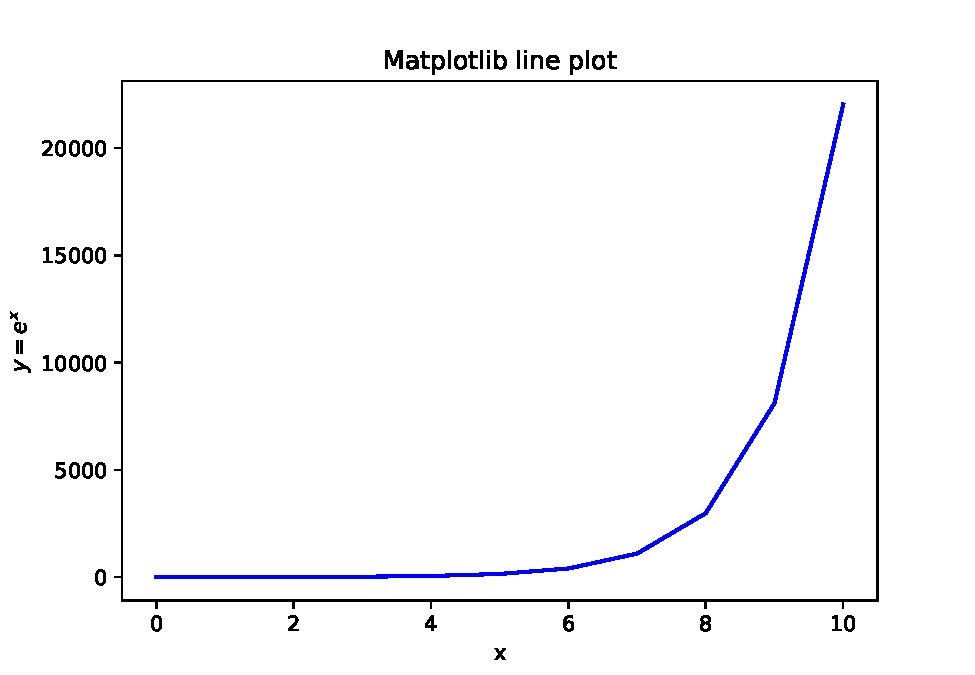
\includegraphics{Toolbox_files/figure-latex/lib-py-1.pdf}

\begin{Shaded}
\begin{Highlighting}[]
\CommentTok{\# create an instance of a linear regression model where we will estimate the intercept}
\NormalTok{model }\OperatorTok{=}\NormalTok{ linear\_model.LinearRegression(fit\_intercept }\OperatorTok{=} \VariableTok{True}\NormalTok{)}
\end{Highlighting}
\end{Shaded}

{\texttt{scikit-learn} requires that the features (x) be a matrix and the response y be a one-dimension array.}

\hypertarget{prepare-x}{%
\subsection{Prepare X}\label{prepare-x}}

\begin{Shaded}
\begin{Highlighting}[]
\CommentTok{\# Create an X matrix using the x values}
\NormalTok{x }\OperatorTok{=}\NormalTok{ olympic.year.values}
\NormalTok{x.shape}
\end{Highlighting}
\end{Shaded}

\begin{verbatim}
## (28,)
\end{verbatim}

\begin{Shaded}
\begin{Highlighting}[]
\BuiltInTok{type}\NormalTok{(x)}
\end{Highlighting}
\end{Shaded}

\begin{verbatim}
## <class 'numpy.ndarray'>
\end{verbatim}

\begin{Shaded}
\begin{Highlighting}[]
\NormalTok{X }\OperatorTok{=}\NormalTok{ x.reshape([}\OperatorTok{{-}}\DecValTok{1}\NormalTok{, }\DecValTok{1}\NormalTok{]) }\CommentTok{\# here {-} 1 means "I don\textquotesingle{}t know how many..."}
\end{Highlighting}
\end{Shaded}

\begin{Shaded}
\begin{Highlighting}[]
\CommentTok{\# if you know the dimensions}
\NormalTok{X }\OperatorTok{=}\NormalTok{ x.reshape((}\DecValTok{28}\NormalTok{, }\DecValTok{1}\NormalTok{))}
\end{Highlighting}
\end{Shaded}

\begin{Shaded}
\begin{Highlighting}[]
\CommentTok{\# Check the shape}
\BuiltInTok{print}\NormalTok{(X.shape)}
\end{Highlighting}
\end{Shaded}

\begin{verbatim}
## (28, 1)
\end{verbatim}

Alternative? Try the following

\begin{Shaded}
\begin{Highlighting}[]
\NormalTok{X2 }\OperatorTok{=}\NormalTok{ olympic[[}\StringTok{\textquotesingle{}year\textquotesingle{}}\NormalTok{]]}
\NormalTok{X2.shape}
\end{Highlighting}
\end{Shaded}

\begin{verbatim}
## (28, 1)
\end{verbatim}

\hypertarget{prepare-y}{%
\subsection{Prepare y}\label{prepare-y}}

\begin{Shaded}
\begin{Highlighting}[]
\NormalTok{y }\OperatorTok{=}\NormalTok{ olympic.time}
\NormalTok{y.shape}
\end{Highlighting}
\end{Shaded}

\begin{verbatim}
## (28,)
\end{verbatim}

\begin{Shaded}
\begin{Highlighting}[]
\BuiltInTok{type}\NormalTok{(y)}\CommentTok{\# fine! note the difference between year and time; we had to reshape year}
\end{Highlighting}
\end{Shaded}

\begin{verbatim}
## <class 'pandas.core.series.Series'>
\end{verbatim}

\hypertarget{fit}{%
\subsection{Fit}\label{fit}}

\begin{Shaded}
\begin{Highlighting}[]
\CommentTok{\# Now fit the model}
\NormalTok{model.fit(X, y)}
\end{Highlighting}
\end{Shaded}

\begin{verbatim}
## LinearRegression()
\end{verbatim}

\begin{Shaded}
\begin{Highlighting}[]
\BuiltInTok{print}\NormalTok{(model.coef\_) }\CommentTok{\# coefficient}
\end{Highlighting}
\end{Shaded}

\begin{verbatim}
## [-0.01327532]
\end{verbatim}

\begin{Shaded}
\begin{Highlighting}[]
\BuiltInTok{print}\NormalTok{(model.intercept\_) }\CommentTok{\# intercept}
\end{Highlighting}
\end{Shaded}

\begin{verbatim}
## 36.30912040967222
\end{verbatim}

\hypertarget{prediction}{%
\subsection{Prediction}\label{prediction}}

\begin{Shaded}
\begin{Highlighting}[]
\CommentTok{\# New X as np array}
\NormalTok{prediction\_x }\OperatorTok{=}\NormalTok{ np.linspace(}\DecValTok{1900}\NormalTok{, }\DecValTok{2000}\NormalTok{, }\DecValTok{101}\NormalTok{)}
\CommentTok{\# reshape it}
\NormalTok{prediction\_x }\OperatorTok{=}\NormalTok{ prediction\_x.reshape([}\OperatorTok{{-}}\DecValTok{1}\NormalTok{, }\DecValTok{1}\NormalTok{]) }\CommentTok{\# recall {-}1 stands for "i don\textquotesingle{}t know"}
\end{Highlighting}
\end{Shaded}

\begin{Shaded}
\begin{Highlighting}[]
\NormalTok{model.predict(prediction\_x)}
\end{Highlighting}
\end{Shaded}

\begin{verbatim}
## array([11.08600515, 11.07272982, 11.0594545 , 11.04617918, 11.03290385,
##        11.01962853, 11.00635321, 10.99307788, 10.97980256, 10.96652723,
##        10.95325191, 10.93997659, 10.92670126, 10.91342594, 10.90015061,
##        10.88687529, 10.87359997, 10.86032464, 10.84704932, 10.833774  ,
##        10.82049867, 10.80722335, 10.79394802, 10.7806727 , 10.76739738,
##        10.75412205, 10.74084673, 10.72757141, 10.71429608, 10.70102076,
##        10.68774543, 10.67447011, 10.66119479, 10.64791946, 10.63464414,
##        10.62136881, 10.60809349, 10.59481817, 10.58154284, 10.56826752,
##        10.5549922 , 10.54171687, 10.52844155, 10.51516622, 10.5018909 ,
##        10.48861558, 10.47534025, 10.46206493, 10.4487896 , 10.43551428,
##        10.42223896, 10.40896363, 10.39568831, 10.38241299, 10.36913766,
##        10.35586234, 10.34258701, 10.32931169, 10.31603637, 10.30276104,
##        10.28948572, 10.2762104 , 10.26293507, 10.24965975, 10.23638442,
##        10.2231091 , 10.20983378, 10.19655845, 10.18328313, 10.1700078 ,
##        10.15673248, 10.14345716, 10.13018183, 10.11690651, 10.10363119,
##        10.09035586, 10.07708054, 10.06380521, 10.05052989, 10.03725457,
##        10.02397924, 10.01070392,  9.99742859,  9.98415327,  9.97087795,
##         9.95760262,  9.9443273 ,  9.93105198,  9.91777665,  9.90450133,
##         9.891226  ,  9.87795068,  9.86467536,  9.85140003,  9.83812471,
##         9.82484939,  9.81157406,  9.79829874,  9.78502341,  9.77174809,
##         9.75847277])
\end{verbatim}

\hypertarget{scatter-plot-actual-vs-fitted}{%
\subsection{Scatter Plot: Actual vs Fitted}\label{scatter-plot-actual-vs-fitted}}

\begin{Shaded}
\begin{Highlighting}[]
\NormalTok{plt.scatter(x, y)}
\end{Highlighting}
\end{Shaded}

\begin{verbatim}
## <matplotlib.collections.PathCollection object at 0x0000000041C79048>
\end{verbatim}

\begin{Shaded}
\begin{Highlighting}[]
\NormalTok{plt.plot(prediction\_x, model.predict(prediction\_x), color }\OperatorTok{=} \StringTok{\textquotesingle{}red\textquotesingle{}}\NormalTok{)}
\end{Highlighting}
\end{Shaded}

\begin{verbatim}
## [<matplotlib.lines.Line2D object at 0x0000000041C79358>]
\end{verbatim}

\begin{Shaded}
\begin{Highlighting}[]
\NormalTok{plt.show()}
\end{Highlighting}
\end{Shaded}

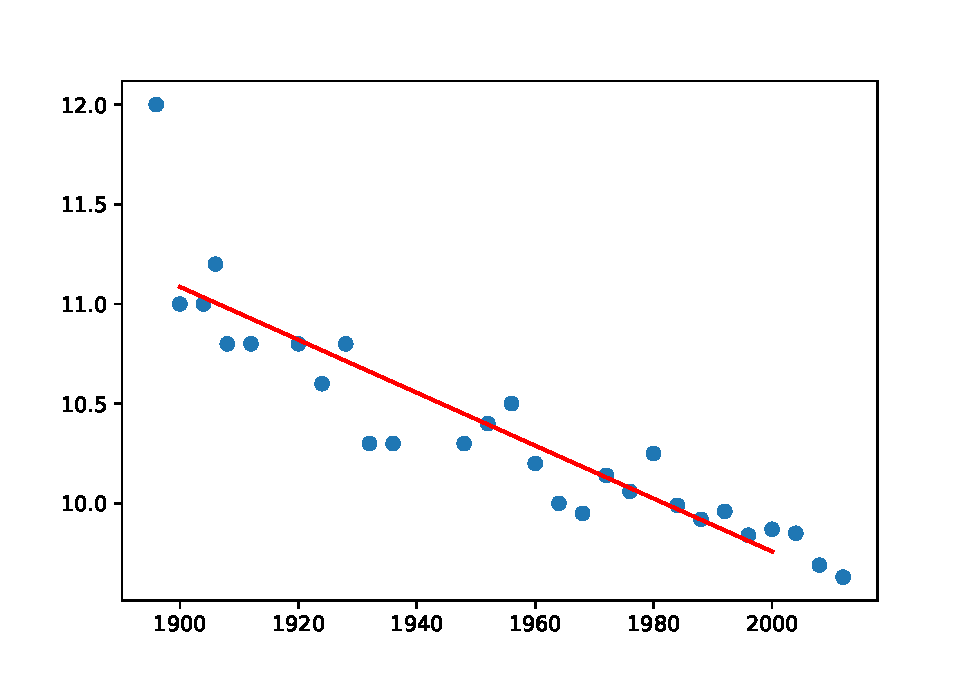
\includegraphics{Toolbox_files/figure-latex/lib-py-3.pdf}

\hypertarget{residual-plot}{%
\subsection{Residual Plot}\label{residual-plot}}

\begin{Shaded}
\begin{Highlighting}[]
\CommentTok{\# find residuals}
\NormalTok{residuals }\OperatorTok{=}\NormalTok{ y }\OperatorTok{{-}}\NormalTok{ model.predict(X)}
\NormalTok{np.mean(residuals) }\CommentTok{\# check mean}
\end{Highlighting}
\end{Shaded}

\begin{verbatim}
## 1.9032394707859825e-16
\end{verbatim}

\begin{Shaded}
\begin{Highlighting}[]
\NormalTok{plt.hist(residuals)}
\end{Highlighting}
\end{Shaded}

\begin{verbatim}
## (array([2., 6., 7., 8., 4., 0., 0., 0., 0., 1.]), array([-0.36119479, -0.23898595, -0.11677712,  0.00543172,  0.12764055,
##         0.24984939,  0.37205822,  0.49426705,  0.61647589,  0.73868472,
##         0.86089356]), <a list of 10 Patch objects>)
\end{verbatim}

\begin{Shaded}
\begin{Highlighting}[]
\NormalTok{plt.show()}
\end{Highlighting}
\end{Shaded}

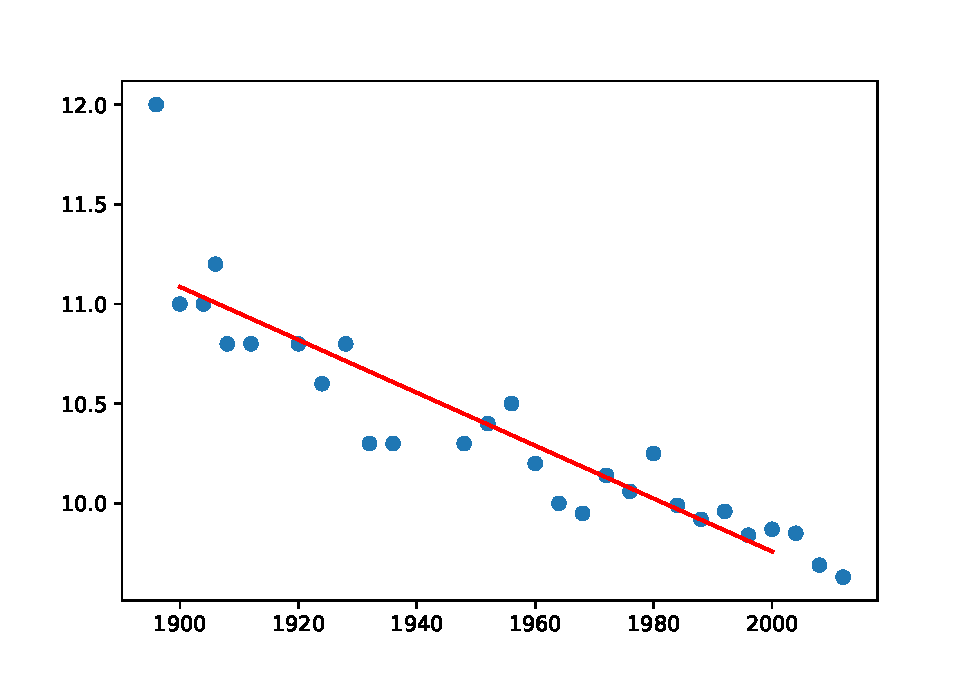
\includegraphics{Toolbox_files/figure-latex/lib-py-5.pdf}

\begin{Shaded}
\begin{Highlighting}[]
\NormalTok{plt.plot(x, residuals, }\StringTok{"o"}\NormalTok{)}
\end{Highlighting}
\end{Shaded}

\begin{verbatim}
## [<matplotlib.lines.Line2D object at 0x0000000041D14F60>]
\end{verbatim}

\begin{Shaded}
\begin{Highlighting}[]
\NormalTok{plt.show()}
\end{Highlighting}
\end{Shaded}

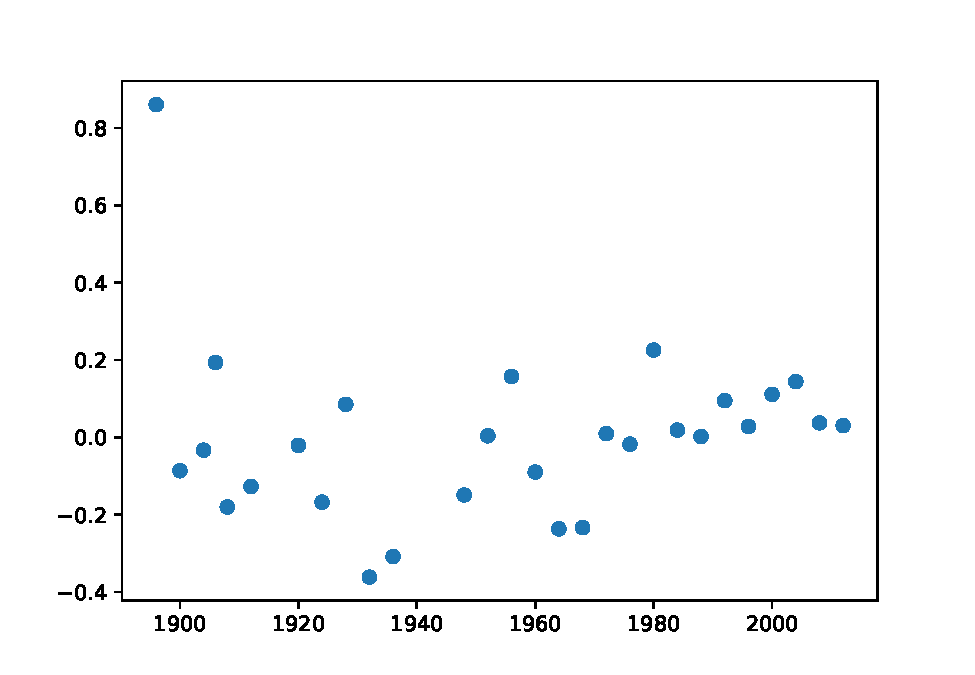
\includegraphics{Toolbox_files/figure-latex/lib-py-6.pdf}

\hypertarget{train-test}{%
\section{Train-Test}\label{train-test}}

\begin{Shaded}
\begin{Highlighting}[]
\ImportTok{import}\NormalTok{ numpy }\ImportTok{as}\NormalTok{ np}
\ImportTok{import}\NormalTok{ pandas }\ImportTok{as}\NormalTok{ pd}
\ImportTok{import}\NormalTok{ matplotlib.pyplot }\ImportTok{as}\NormalTok{ plt}
\ImportTok{from}\NormalTok{ sklearn }\ImportTok{import}\NormalTok{ linear\_model, preprocessing, model\_selection}
\ImportTok{from}\NormalTok{ sklearn.model\_selection }\ImportTok{import}\NormalTok{ train\_test\_split, cross\_val\_score}
\end{Highlighting}
\end{Shaded}

\texttt{train\_test\_split()} takes a list of arrays and splits each array into two arrays (a training set and a test set) by randomly selecting rows or values.

\hypertarget{example}{%
\subsection{Example}\label{example}}

\begin{Shaded}
\begin{Highlighting}[]
\CommentTok{\# x is our predictor matrix}
\NormalTok{X }\OperatorTok{=}\NormalTok{ np.arange(}\DecValTok{20}\NormalTok{).reshape((}\DecValTok{2}\NormalTok{, }\OperatorTok{{-}}\DecValTok{1}\NormalTok{)).T}
\BuiltInTok{print}\NormalTok{(X)}
\end{Highlighting}
\end{Shaded}

\begin{verbatim}
## [[ 0 10]
##  [ 1 11]
##  [ 2 12]
##  [ 3 13]
##  [ 4 14]
##  [ 5 15]
##  [ 6 16]
##  [ 7 17]
##  [ 8 18]
##  [ 9 19]]
\end{verbatim}

\begin{Shaded}
\begin{Highlighting}[]
\CommentTok{\# y is a numeric output {-} for regression methods}
\NormalTok{y }\OperatorTok{=}\NormalTok{ np.arange(}\DecValTok{10}\NormalTok{)}
\BuiltInTok{print}\NormalTok{(y)}
\end{Highlighting}
\end{Shaded}

\begin{verbatim}
## [0 1 2 3 4 5 6 7 8 9]
\end{verbatim}

\begin{Shaded}
\begin{Highlighting}[]
\CommentTok{\# z is a categorical output {-} for classification methods}
\NormalTok{z }\OperatorTok{=}\NormalTok{ np.array([}\DecValTok{0}\NormalTok{,}\DecValTok{0}\NormalTok{,}\DecValTok{0}\NormalTok{,}\DecValTok{0}\NormalTok{,}\DecValTok{0}\NormalTok{,}\DecValTok{1}\NormalTok{,}\DecValTok{1}\NormalTok{,}\DecValTok{1}\NormalTok{,}\DecValTok{1}\NormalTok{,}\DecValTok{1}\NormalTok{])}
\BuiltInTok{print}\NormalTok{(z)}
\end{Highlighting}
\end{Shaded}

\begin{verbatim}
## [0 0 0 0 0 1 1 1 1 1]
\end{verbatim}

We can use \texttt{train\_test\_split()} on each array \textbf{individually}.

What happens?

\begin{Shaded}
\begin{Highlighting}[]
\NormalTok{train\_test\_split(X, test\_size }\OperatorTok{=} \DecValTok{1}\OperatorTok{/}\DecValTok{4}\NormalTok{, random\_state }\OperatorTok{=} \DecValTok{1}\NormalTok{)}
\end{Highlighting}
\end{Shaded}

\begin{verbatim}
## [array([[ 4, 14],
##        [ 0, 10],
##        [ 3, 13],
##        [ 1, 11],
##        [ 7, 17],
##        [ 8, 18],
##        [ 5, 15]]), array([[ 2, 12],
##        [ 9, 19],
##        [ 6, 16]])]
\end{verbatim}

\begin{Shaded}
\begin{Highlighting}[]
\BuiltInTok{type}\NormalTok{(train\_test\_split(X, test\_size }\OperatorTok{=} \DecValTok{1}\OperatorTok{/}\DecValTok{4}\NormalTok{, random\_state }\OperatorTok{=} \DecValTok{1}\NormalTok{))}
\end{Highlighting}
\end{Shaded}

\begin{verbatim}
## <class 'list'>
\end{verbatim}

Store them

\begin{Shaded}
\begin{Highlighting}[]
\NormalTok{X\_train, X\_test }\OperatorTok{=}\NormalTok{ train\_test\_split(X, test\_size }\OperatorTok{=} \DecValTok{1}\OperatorTok{/}\DecValTok{4}\NormalTok{, random\_state }\OperatorTok{=} \DecValTok{1}\NormalTok{)}
\BuiltInTok{print}\NormalTok{(X\_train)}
\end{Highlighting}
\end{Shaded}

\begin{verbatim}
## [[ 4 14]
##  [ 0 10]
##  [ 3 13]
##  [ 1 11]
##  [ 7 17]
##  [ 8 18]
##  [ 5 15]]
\end{verbatim}

\begin{Shaded}
\begin{Highlighting}[]
\BuiltInTok{print}\NormalTok{(X\_test)}
\end{Highlighting}
\end{Shaded}

\begin{verbatim}
## [[ 2 12]
##  [ 9 19]
##  [ 6 16]]
\end{verbatim}

\begin{Shaded}
\begin{Highlighting}[]
\NormalTok{y\_train, y\_test }\OperatorTok{=}\NormalTok{ train\_test\_split(y, test\_size }\OperatorTok{=} \DecValTok{1}\OperatorTok{/}\DecValTok{4}\NormalTok{, random\_state }\OperatorTok{=} \DecValTok{1}\NormalTok{)}
\BuiltInTok{print}\NormalTok{(y\_train)}
\end{Highlighting}
\end{Shaded}

\begin{verbatim}
## [4 0 3 1 7 8 5]
\end{verbatim}

\begin{Shaded}
\begin{Highlighting}[]
\BuiltInTok{print}\NormalTok{(y\_test)}
\end{Highlighting}
\end{Shaded}

\begin{verbatim}
## [2 9 6]
\end{verbatim}

We can also apply it to multiple arrays \textbf{simultaneously}.

\begin{Shaded}
\begin{Highlighting}[]
\NormalTok{X\_train, X\_test, y\_train, y\_test }\OperatorTok{=}\NormalTok{ train\_test\_split(X, y, test\_size }\OperatorTok{=} \DecValTok{1}\OperatorTok{/}\DecValTok{4}\NormalTok{, random\_state }\OperatorTok{=} \DecValTok{1}\NormalTok{)}
\BuiltInTok{print}\NormalTok{(X\_train)}
\end{Highlighting}
\end{Shaded}

\begin{verbatim}
## [[ 4 14]
##  [ 0 10]
##  [ 3 13]
##  [ 1 11]
##  [ 7 17]
##  [ 8 18]
##  [ 5 15]]
\end{verbatim}

\begin{Shaded}
\begin{Highlighting}[]
\BuiltInTok{print}\NormalTok{(X\_test)}
\end{Highlighting}
\end{Shaded}

\begin{verbatim}
## [[ 2 12]
##  [ 9 19]
##  [ 6 16]]
\end{verbatim}

\begin{Shaded}
\begin{Highlighting}[]
\BuiltInTok{print}\NormalTok{(y\_train)}
\end{Highlighting}
\end{Shaded}

\begin{verbatim}
## [4 0 3 1 7 8 5]
\end{verbatim}

\begin{Shaded}
\begin{Highlighting}[]
\BuiltInTok{print}\NormalTok{(y\_test)}
\end{Highlighting}
\end{Shaded}

\begin{verbatim}
## [2 9 6]
\end{verbatim}

If you have a \textbf{categorical} variable, the \texttt{stratify} argument ensures
that you'll get an appropriate number of each category in the resulting split.
For this purpose, we previously created \texttt{z}.

\begin{Shaded}
\begin{Highlighting}[]
\NormalTok{X\_train, X\_test, z\_train, z\_test }\OperatorTok{=}\NormalTok{ train\_test\_split(}
\NormalTok{  X, z, test\_size }\OperatorTok{=} \DecValTok{1}\OperatorTok{/}\DecValTok{4}\NormalTok{, random\_state }\OperatorTok{=} \DecValTok{1}\NormalTok{, stratify }\OperatorTok{=}\NormalTok{ z}
\NormalTok{)}
\end{Highlighting}
\end{Shaded}

\begin{Shaded}
\begin{Highlighting}[]
\BuiltInTok{print}\NormalTok{(X\_train)}
\end{Highlighting}
\end{Shaded}

\begin{verbatim}
## [[ 4 14]
##  [ 0 10]
##  [ 5 15]
##  [ 7 17]
##  [ 1 11]
##  [ 9 19]
##  [ 2 12]]
\end{verbatim}

\begin{Shaded}
\begin{Highlighting}[]
\BuiltInTok{print}\NormalTok{(X\_test)}
\end{Highlighting}
\end{Shaded}

\begin{verbatim}
## [[ 3 13]
##  [ 8 18]
##  [ 6 16]]
\end{verbatim}

\begin{Shaded}
\begin{Highlighting}[]
\BuiltInTok{print}\NormalTok{(z\_train)}
\end{Highlighting}
\end{Shaded}

\begin{verbatim}
## [0 0 1 1 0 1 0]
\end{verbatim}

\begin{Shaded}
\begin{Highlighting}[]
\BuiltInTok{print}\NormalTok{(z\_test)}
\end{Highlighting}
\end{Shaded}

\begin{verbatim}
## [0 1 1]
\end{verbatim}

\hypertarget{another-example}{%
\subsection{Another Example}\label{another-example}}

\begin{Shaded}
\begin{Highlighting}[]
\CommentTok{\# Example data: ironslag}
\NormalTok{iron }\OperatorTok{=}\NormalTok{ pd.read\_csv(}\StringTok{\textquotesingle{}https://raw.githubusercontent.com/bhaswar{-}chakma/toolbox/main/data/ironslag.csv\textquotesingle{}}\NormalTok{)}
\end{Highlighting}
\end{Shaded}

\begin{Shaded}
\begin{Highlighting}[]
\NormalTok{iron.head()}
\end{Highlighting}
\end{Shaded}

\begin{verbatim}
##    chemical  magnetic
## 0        24        25
## 1        16        22
## 2        24        17
## 3        18        21
## 4        18        20
\end{verbatim}

\begin{Shaded}
\begin{Highlighting}[]
\NormalTok{iron.shape}
\end{Highlighting}
\end{Shaded}

\begin{verbatim}
## (53, 2)
\end{verbatim}

\emph{Magnetic test is cheaper; chemical test is more accurate.Can we use the magnetic test to predict the chemical test result?}

\begin{itemize}
\item
  \texttt{X} = magnetic test result
\item
  \texttt{y} = chemical test
\end{itemize}

\begin{Shaded}
\begin{Highlighting}[]
\NormalTok{plt.scatter(iron.magnetic, iron.chemical)}
\end{Highlighting}
\end{Shaded}

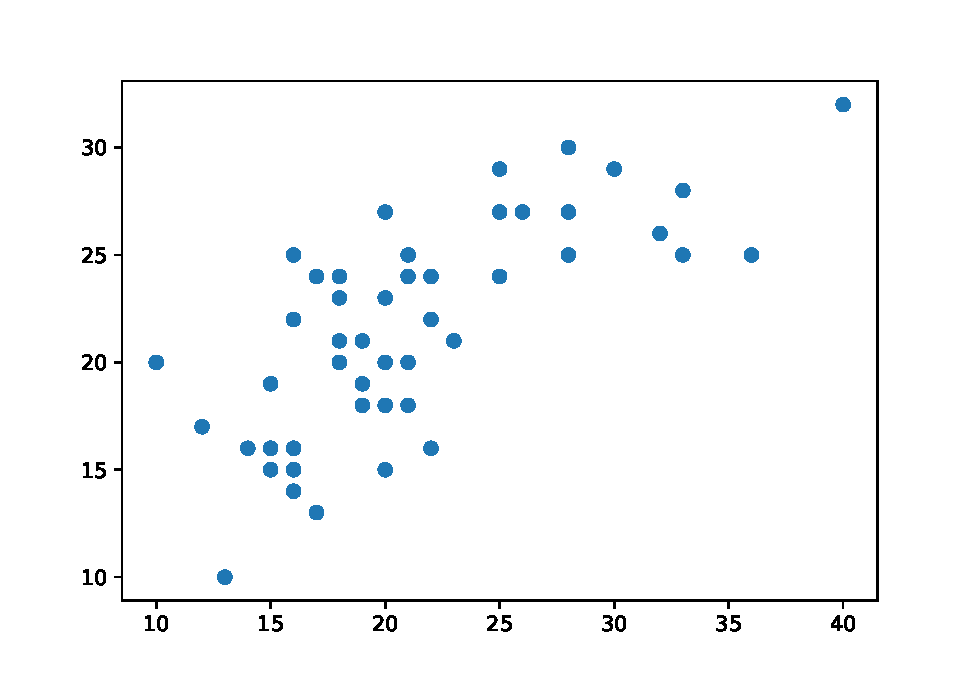
\includegraphics{Toolbox_files/figure-latex/lib-py-9.pdf}

\textbf{Create a hold-out set using train-test split}

\begin{Shaded}
\begin{Highlighting}[]
\NormalTok{train, test }\OperatorTok{=}\NormalTok{ train\_test\_split(}
\NormalTok{  iron, test\_size }\OperatorTok{=} \DecValTok{1}\OperatorTok{/}\DecValTok{5}\NormalTok{, random\_state }\OperatorTok{=} \DecValTok{1}
\NormalTok{)}
\end{Highlighting}
\end{Shaded}

\begin{Shaded}
\begin{Highlighting}[]
\NormalTok{train.shape}
\end{Highlighting}
\end{Shaded}

\begin{verbatim}
## (42, 2)
\end{verbatim}

\begin{Shaded}
\begin{Highlighting}[]
\NormalTok{train.head()}
\end{Highlighting}
\end{Shaded}

\begin{verbatim}
##     chemical  magnetic
## 3         18        21
## 21        13        17
## 49        25        36
## 38        23        18
## 41        15        16
\end{verbatim}

\begin{Shaded}
\begin{Highlighting}[]
\NormalTok{test.shape}
\end{Highlighting}
\end{Shaded}

\begin{verbatim}
## (11, 2)
\end{verbatim}

\begin{Shaded}
\begin{Highlighting}[]
\NormalTok{test.head()}
\end{Highlighting}
\end{Shaded}

\begin{verbatim}
##     chemical  magnetic
## 30        27        25
## 2         24        17
## 51        28        33
## 32        20        18
## 31        22        22
\end{verbatim}

\begin{Shaded}
\begin{Highlighting}[]
\NormalTok{plt.scatter(train.magnetic, train.chemical)}
\end{Highlighting}
\end{Shaded}

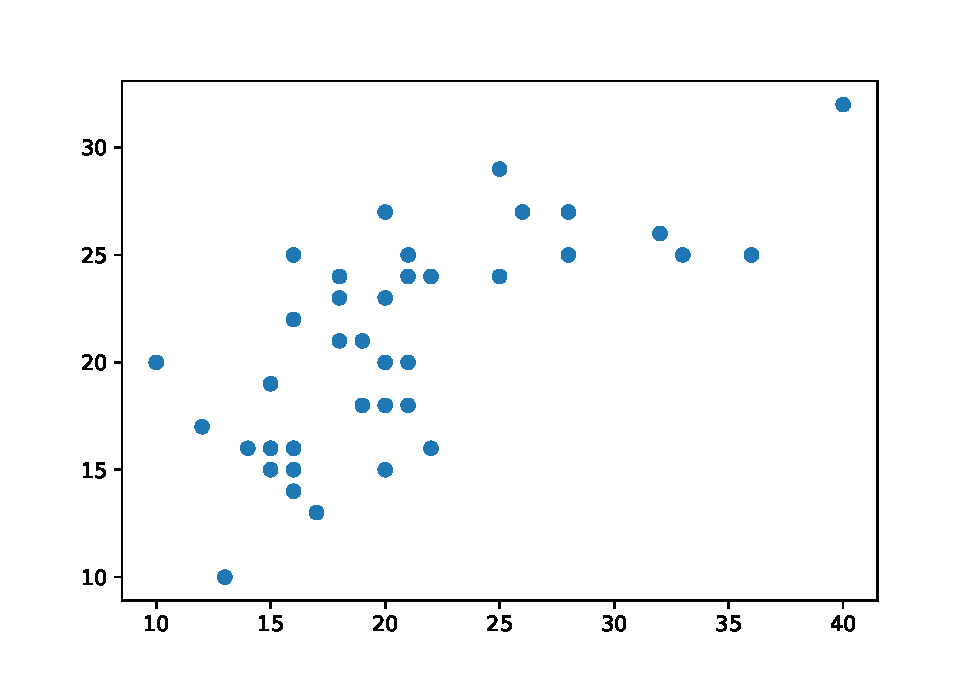
\includegraphics{Toolbox_files/figure-latex/lib-py-11.pdf}

\textbf{Use only the training data to try out possible models}

\begin{Shaded}
\begin{Highlighting}[]
\CommentTok{\# sklearn requires our predictor variables to be in a two dimensional array}
\CommentTok{\# reshape to have 1 column}
\CommentTok{\# the {-}1 in reshape means I don\textquotesingle{}t want to figure out all the necessary dimensions}
\CommentTok{\# i want 1 column, and numpy, you figure out how many rows I need}
\NormalTok{X }\OperatorTok{=}\NormalTok{ train.magnetic.values.reshape(}\OperatorTok{{-}}\DecValTok{1}\NormalTok{,}\DecValTok{1}\NormalTok{)}
\NormalTok{X.shape}
\end{Highlighting}
\end{Shaded}

\begin{verbatim}
## (42, 1)
\end{verbatim}

\begin{Shaded}
\begin{Highlighting}[]
\NormalTok{y }\OperatorTok{=}\NormalTok{ train.chemical.values}
\NormalTok{y.shape}
\end{Highlighting}
\end{Shaded}

\begin{verbatim}
## (42,)
\end{verbatim}

\begin{Shaded}
\begin{Highlighting}[]
\NormalTok{np.corrcoef(train.magnetic.values, train.chemical.values)}
\end{Highlighting}
\end{Shaded}

\begin{verbatim}
## array([[1.        , 0.70876994],
##        [0.70876994, 1.        ]])
\end{verbatim}

\begin{Shaded}
\begin{Highlighting}[]
\CommentTok{\# r{-}squared}
\NormalTok{np.corrcoef(train.magnetic.values, train.chemical.values)[}\DecValTok{0}\NormalTok{,}\DecValTok{1}\NormalTok{] }\OperatorTok{**} \DecValTok{2}
\end{Highlighting}
\end{Shaded}

\begin{verbatim}
## 0.5023548215592254
\end{verbatim}

\textbf{Fit a linear model between x and y}

\begin{Shaded}
\begin{Highlighting}[]
\NormalTok{linear }\OperatorTok{=}\NormalTok{ linear\_model.LinearRegression()}
\NormalTok{linear.fit(X, y)}
\end{Highlighting}
\end{Shaded}

\begin{verbatim}
## LinearRegression()
\end{verbatim}

\texttt{linear.score()} is the \(R^2\) value.

\begin{Shaded}
\begin{Highlighting}[]
\CommentTok{\# linear.score is the R\^{}2 value}
\CommentTok{\# how much error is reduced from no model (variance or MSE)}
\CommentTok{\# vs having the regression model}
\NormalTok{linear.score(X, y)}
\end{Highlighting}
\end{Shaded}

\begin{verbatim}
## 0.5023548215592256
\end{verbatim}

\begin{Shaded}
\begin{Highlighting}[]
\NormalTok{x\_predict }\OperatorTok{=}\NormalTok{ np.arange(}\DecValTok{10}\NormalTok{, }\DecValTok{40}\NormalTok{).reshape(}\OperatorTok{{-}}\DecValTok{1}\NormalTok{,}\DecValTok{1}\NormalTok{) }\CommentTok{\# values to be used for prediction}
\NormalTok{lin\_y\_hat }\OperatorTok{=}\NormalTok{ linear.predict(x\_predict) }\CommentTok{\# use the values and predict}
\end{Highlighting}
\end{Shaded}

\begin{Shaded}
\begin{Highlighting}[]
\NormalTok{plt.scatter(X, y)}
\end{Highlighting}
\end{Shaded}

\begin{verbatim}
## <matplotlib.collections.PathCollection object at 0x0000000004BFF2B0>
\end{verbatim}

\begin{Shaded}
\begin{Highlighting}[]
\NormalTok{plt.plot(x\_predict, lin\_y\_hat, c }\OperatorTok{=} \StringTok{\textquotesingle{}red\textquotesingle{}}\NormalTok{)}
\end{Highlighting}
\end{Shaded}

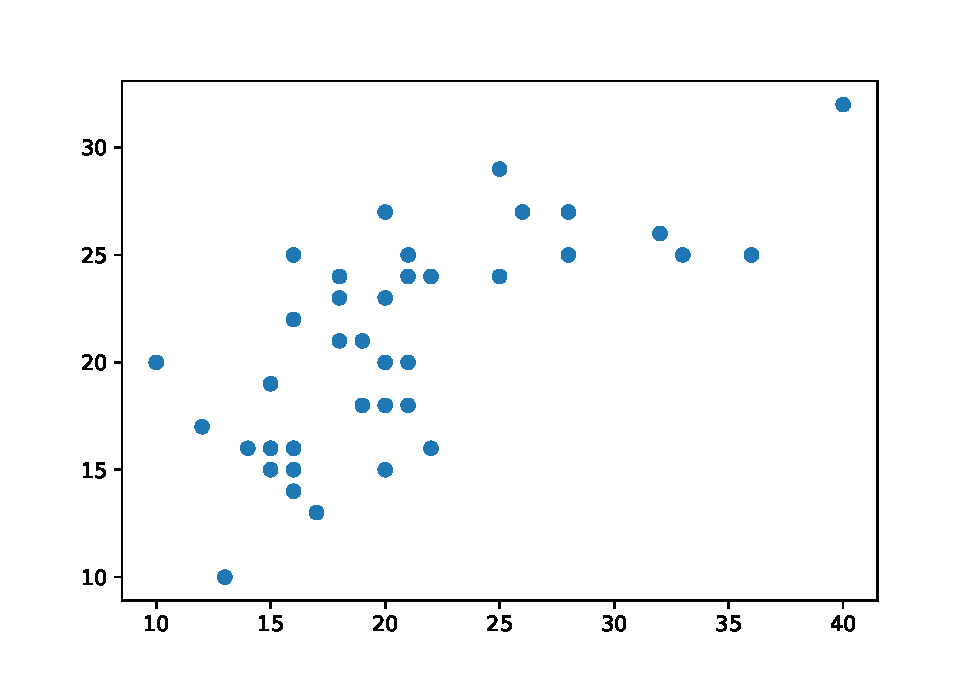
\includegraphics{Toolbox_files/figure-latex/lib-py-13.pdf}

\hypertarget{cross-validation}{%
\section{Cross Validation}\label{cross-validation}}

\textbf{Linear Model}

\begin{Shaded}
\begin{Highlighting}[]
\CommentTok{\# shuffle split says \textquotesingle{}shuffle the data\textquotesingle{} and split it into 5 equal parts}
\NormalTok{cv }\OperatorTok{=}\NormalTok{ model\_selection.ShuffleSplit(n\_splits }\OperatorTok{=} \DecValTok{5}\NormalTok{, test\_size }\OperatorTok{=} \FloatTok{0.3}\NormalTok{, random\_state}\OperatorTok{=}\DecValTok{0}\NormalTok{)}
\NormalTok{cv\_linear }\OperatorTok{=}\NormalTok{ model\_selection.cross\_val\_score(linear, X, y, cv }\OperatorTok{=}\NormalTok{ cv)}
\BuiltInTok{print}\NormalTok{(cv\_linear)}
\end{Highlighting}
\end{Shaded}

\begin{verbatim}
## [0.5811901  0.5322723  0.45145614 0.13698027 0.65315849]
\end{verbatim}

\begin{Shaded}
\begin{Highlighting}[]
\BuiltInTok{print}\NormalTok{(np.mean(cv\_linear))}
\end{Highlighting}
\end{Shaded}

\begin{verbatim}
## 0.4710114602819653
\end{verbatim}

\textbf{Polynomial Fit - Quadratic}

\begin{Shaded}
\begin{Highlighting}[]
\CommentTok{\# preprocessing polynomial features creates a polynomial based on X}
\NormalTok{quad }\OperatorTok{=}\NormalTok{ preprocessing.PolynomialFeatures(}\DecValTok{2}\NormalTok{)}
\NormalTok{quadX }\OperatorTok{=}\NormalTok{ quad.fit\_transform(X)}
\NormalTok{quad\_model }\OperatorTok{=}\NormalTok{ linear\_model.LinearRegression()}
\NormalTok{quad\_model.fit(quadX, y)}
\end{Highlighting}
\end{Shaded}

\begin{verbatim}
## LinearRegression()
\end{verbatim}

\begin{Shaded}
\begin{Highlighting}[]
\NormalTok{cv\_quad }\OperatorTok{=}\NormalTok{ model\_selection.cross\_val\_score(quad\_model, quadX, y, cv }\OperatorTok{=}\NormalTok{ cv)}
\BuiltInTok{print}\NormalTok{(cv\_quad)}
\end{Highlighting}
\end{Shaded}

\begin{verbatim}
## [ 0.20489832  0.39310396  0.24068822 -0.11114126  0.58637808]
\end{verbatim}

\begin{Shaded}
\begin{Highlighting}[]
\BuiltInTok{print}\NormalTok{(np.mean(cv\_quad))}
\end{Highlighting}
\end{Shaded}

\begin{verbatim}
## 0.2627854641006778
\end{verbatim}

\textbf{Cubic Fit}

\begin{Shaded}
\begin{Highlighting}[]
\NormalTok{cube }\OperatorTok{=}\NormalTok{ preprocessing.PolynomialFeatures(}\DecValTok{3}\NormalTok{)}
\NormalTok{cubeX }\OperatorTok{=}\NormalTok{ cube.fit\_transform(X)}
\NormalTok{cube\_model }\OperatorTok{=}\NormalTok{ linear\_model.LinearRegression()}
\NormalTok{cube\_model.fit(cubeX, y)}
\end{Highlighting}
\end{Shaded}

\begin{verbatim}
## LinearRegression()
\end{verbatim}

\begin{Shaded}
\begin{Highlighting}[]
\NormalTok{cv\_cube }\OperatorTok{=}\NormalTok{ model\_selection.cross\_val\_score(cube\_model, cubeX, y, cv }\OperatorTok{=}\NormalTok{ cv)}
\BuiltInTok{print}\NormalTok{(cv\_cube)}
\end{Highlighting}
\end{Shaded}

\begin{verbatim}
## [-0.01197637 -0.80626221  0.08937258 -0.2144141  -0.62784165]
\end{verbatim}

\begin{Shaded}
\begin{Highlighting}[]
\BuiltInTok{print}\NormalTok{(np.mean(cv\_cube))}
\end{Highlighting}
\end{Shaded}

\begin{verbatim}
## -0.3142243517318586
\end{verbatim}

\textbf{Y \textasciitilde{} log X model}

\begin{Shaded}
\begin{Highlighting}[]
\NormalTok{log\_transform }\OperatorTok{=}\NormalTok{ preprocessing.FunctionTransformer(np.log)}
\NormalTok{logX }\OperatorTok{=}\NormalTok{ log\_transform.fit\_transform(X)}
\NormalTok{logX\_model }\OperatorTok{=}\NormalTok{ linear\_model.LinearRegression()}
\NormalTok{logX\_model.fit(logX, y)}
\end{Highlighting}
\end{Shaded}

\begin{verbatim}
## LinearRegression()
\end{verbatim}

\begin{Shaded}
\begin{Highlighting}[]
\NormalTok{cv\_logX }\OperatorTok{=}\NormalTok{ model\_selection.cross\_val\_score(logX\_model, logX, y, cv }\OperatorTok{=}\NormalTok{ cv)}
\BuiltInTok{print}\NormalTok{(cv\_logX)}
\end{Highlighting}
\end{Shaded}

\begin{verbatim}
## [ 0.47681194  0.52326867  0.36527782 -0.08925939  0.61651106]
\end{verbatim}

\begin{Shaded}
\begin{Highlighting}[]
\BuiltInTok{print}\NormalTok{(np.mean(cv\_logX))}
\end{Highlighting}
\end{Shaded}

\begin{verbatim}
## 0.3785220199147977
\end{verbatim}

\hypertarget{r-strings}{%
\chapter{R Strings}\label{r-strings}}

\hypertarget{string-manupulation-with-base-r-functions}{%
\section{String Manupulation with Base R Functions}\label{string-manupulation-with-base-r-functions}}

There are many functions in base R for basic string manipulation.

Function

Example

{\textbf{\texttt{nchar()}
}}

\begin{Shaded}
\begin{Highlighting}[]
\NormalTok{y }\OtherTok{\textless{}{-}} \FunctionTok{c}\NormalTok{(}\StringTok{"Hello"}\NormalTok{, }\StringTok{"World"}\NormalTok{, }\StringTok{"Hello"}\NormalTok{, }\StringTok{"Universe"}\NormalTok{)}
\FunctionTok{nchar}\NormalTok{(y) }\CommentTok{\# Returns number of characters}
\end{Highlighting}
\end{Shaded}

\begin{verbatim}
## [1] 5 5 5 8
\end{verbatim}

{\textbf{\texttt{tolower()}
}}

\begin{Shaded}
\begin{Highlighting}[]
\FunctionTok{tolower}\NormalTok{(y)}
\end{Highlighting}
\end{Shaded}

\begin{verbatim}
## [1] "hello"    "world"    "hello"    "universe"
\end{verbatim}

{\textbf{\texttt{toupper()}
}}

\begin{Shaded}
\begin{Highlighting}[]
\FunctionTok{toupper}\NormalTok{(y)}
\end{Highlighting}
\end{Shaded}

\begin{verbatim}
## [1] "HELLO"    "WORLD"    "HELLO"    "UNIVERSE"
\end{verbatim}

{\textbf{\texttt{chartr()}
}}

\begin{Shaded}
\begin{Highlighting}[]
\FunctionTok{chartr}\NormalTok{(}\StringTok{"oe"}\NormalTok{, }\StringTok{"$\#"}\NormalTok{, y)}\CommentTok{\#o becomes $; e becomes \#}
\end{Highlighting}
\end{Shaded}

\begin{verbatim}
## [1] "H#ll$"    "W$rld"    "H#ll$"    "Univ#rs#"
\end{verbatim}

{\textbf{\texttt{substr()}
}}

\begin{Shaded}
\begin{Highlighting}[]
\NormalTok{x }\OtherTok{\textless{}{-}} \StringTok{"1t345s?"}
\FunctionTok{substr}\NormalTok{(x, }\DecValTok{2}\NormalTok{, }\DecValTok{6}\NormalTok{) }\CommentTok{\# provides strings from 2 to 6}
\end{Highlighting}
\end{Shaded}

\begin{verbatim}
## [1] "t345s"
\end{verbatim}

{\textbf{\texttt{strsplit()}
}}

\begin{Shaded}
\begin{Highlighting}[]
\NormalTok{x }\OtherTok{\textless{}{-}} \StringTok{"R\#Rocks\#!"}
\FunctionTok{strsplit}\NormalTok{(x, }\AttributeTok{split =} \StringTok{"\#"}\NormalTok{)}
\end{Highlighting}
\end{Shaded}

\begin{verbatim}
## [[1]]
## [1] "R"     "Rocks" "!"
\end{verbatim}

\hypertarget{stringr}{%
\section{\texorpdfstring{\texttt{stringr}}{stringr}}\label{stringr}}

\begin{Shaded}
\begin{Highlighting}[]
\FunctionTok{library}\NormalTok{(stringr)}
\end{Highlighting}
\end{Shaded}

\begin{longtable}[]{@{}ccc@{}}
\toprule
Job & stringr & Base R \\
\midrule
\endhead
String concatenation & \texttt{str\_c()} & \texttt{paste()} \\
Number of characters & \texttt{str\_length()} & \texttt{nchar()} \\
Extracts substrings & \texttt{str\_sub()} & \texttt{substr()} \\
Duplicates characters & \texttt{str\_dup()} & \\
Removes leading and trailing whitespace & \texttt{str\_trim()} & \\
Pads a string & \texttt{str\_pad()} & \\
Wraps a string paragraph & \texttt{str\_wrap()} & \\
\bottomrule
\end{longtable}

\hypertarget{regular-expressions}{%
\section{Regular Expressions}\label{regular-expressions}}

A \textbf{regular expression} (or \textbf{regex}) is a set of symbols that describes a text pattern. More formally, a regular expression is a pattern that describes a set of strings.

Regular expressions are a formal language in the sense that the symbols have a defined set of rules to specify the desired patterns.

\hypertarget{stringr-functions-for-regular-expressions}{%
\subsection{\texorpdfstring{\texttt{stringr} Functions for Regular Expressions}{stringr Functions for Regular Expressions}}\label{stringr-functions-for-regular-expressions}}

\begin{longtable}[]{@{}
  >{\centering\arraybackslash}p{(\columnwidth - 2\tabcolsep) * \real{0.25}}
  >{\centering\arraybackslash}p{(\columnwidth - 2\tabcolsep) * \real{0.75}}@{}}
\toprule
Function & Job \\
\midrule
\endhead
\texttt{str\_detect}(str, pattern) & Detects the presence of a pattern and returns TRUE if it is found \\
\texttt{str\_locate}(str, pattern) & Locate the 1st position of a pattern and return a matrix with start \& end.s \\
\texttt{str\_extract}(str, pattern) & Extracts text corresponding to the first match. \\
\texttt{str\_match}(str, pattern) & Extracts capture groups formed by () from the first match. \\
\texttt{str\_split}(str, pattern) & Splits string into pieces and returns a list of character vectors. \\
\bottomrule
\end{longtable}

\hypertarget{sql}{%
\chapter{SQL}\label{sql}}

\hypertarget{create}{%
\section{CREATE}\label{create}}

The general syntax to create a table:

\begin{Shaded}
\begin{Highlighting}[]
\KeywordTok{create} \KeywordTok{table}\NormalTok{ TABLENAME (}
\NormalTok{  COLUMN1 datatype, }
\NormalTok{  COLUMN2 datatype, }
\NormalTok{  COLUMN3 datatype, }
  \OperatorTok{..}\NormalTok{. );}
\end{Highlighting}
\end{Shaded}

To create a table called \texttt{TEST} with two columns - \texttt{ID} of type integer, and \texttt{NAME} of type varchar, we could create it using the following SQL statement:

\begin{Shaded}
\begin{Highlighting}[]
\KeywordTok{create} \KeywordTok{table}\NormalTok{ TEST(}
  \KeywordTok{ID} \DataTypeTok{int}
\NormalTok{  NAME }\DataTypeTok{varchar}\NormalTok{(}\DecValTok{30}\NormalTok{)}
\NormalTok{);}
\end{Highlighting}
\end{Shaded}

To create a table called \texttt{COUNTRY} with an \texttt{ID} column, a two letter country code column \texttt{CCODE}, and a variable length country name column \texttt{NAME}:

\begin{Shaded}
\begin{Highlighting}[]
\KeywordTok{create} \KeywordTok{table}\NormalTok{ COUNTRY(}
    \KeywordTok{ID} \DataTypeTok{int}\NormalTok{,}
\NormalTok{    CCODE }\DataTypeTok{char}\NormalTok{(}\DecValTok{2}\NormalTok{),}
\NormalTok{    NAME }\DataTypeTok{varchar}\NormalTok{(}\DecValTok{60}\NormalTok{)}
\NormalTok{);}
\end{Highlighting}
\end{Shaded}

Sometimes you may see additional keywords in a create table statement:

\begin{Shaded}
\begin{Highlighting}[]
\KeywordTok{create} \KeywordTok{table}\NormalTok{ COUNTRY(}
    \KeywordTok{ID} \DataTypeTok{int} \KeywordTok{NOT} \KeywordTok{NULL}\NormalTok{,}
\NormalTok{    CCODE }\DataTypeTok{char}\NormalTok{(}\DecValTok{2}\NormalTok{),}
\NormalTok{    NAME }\DataTypeTok{varchar}\NormalTok{(}\DecValTok{60}\NormalTok{),}
    \KeywordTok{PRIMARY} \KeywordTok{KEY}\NormalTok{(}\KeywordTok{ID}\NormalTok{)}
\NormalTok{);}
\end{Highlighting}
\end{Shaded}

\begin{itemize}
\item
  In the above example the \texttt{ID} column has the {\textbf{\texttt{NOT\ NULL}}} constraint added after the datatype - meaning that \emph{it cannot contain a NULL or an empty value}.
\item
  If you look at the last row in the create table statement above you will note that we are using \texttt{ID} as a {\textbf{Primary Key}} and the database \textbf{does not allow} Primary Keys to have \textbf{\texttt{NULL}} values. \emph{A Primary Key is a unique identifier in a table, and using Primary Keys can help speed up your queries significantly}.
\item
  If the table you are trying to create already exists in the database, you will get an error indicating table \texttt{XXX.YYY} already exists. To circumvent this error, either create a table with a different name or first \texttt{DROP} the existing table. It is quite common to issue a \texttt{DROP} before doing a \texttt{CREATE} in test and development scenarios.
\end{itemize}

\hypertarget{drop}{%
\section{DROP}\label{drop}}

The general syntax to drop a table:

\begin{Shaded}
\begin{Highlighting}[]
\KeywordTok{drop} \KeywordTok{table}\NormalTok{ TABLENAME;}
\end{Highlighting}
\end{Shaded}

For example, to drop the table COUNTRY, we can use the following code:

\begin{Shaded}
\begin{Highlighting}[]
\KeywordTok{drop} \KeywordTok{table}\NormalTok{ COUNTRY;}
\end{Highlighting}
\end{Shaded}

\hypertarget{alter}{%
\section{ALTER}\label{alter}}

\begin{Shaded}
\begin{Highlighting}[]
\KeywordTok{ALTER} \KeywordTok{TABLE}\NormalTok{ table\_name}
\KeywordTok{ADD} \KeywordTok{COLUMN}\NormalTok{ column\_name data\_type column\_constraint;}

\KeywordTok{ALTER} \KeywordTok{TABLE}\NormalTok{ table\_name}
\KeywordTok{DROP} \KeywordTok{COLUMN}\NormalTok{ column\_name;}

\KeywordTok{ALTER} \KeywordTok{TABLE}\NormalTok{ table\_name}
\KeywordTok{ALTER} \KeywordTok{COLUMN}\NormalTok{ column\_name }\KeywordTok{SET} \KeywordTok{DATA} \KeywordTok{TYPE}\NormalTok{ data\_type;}

\KeywordTok{ALTER} \KeywordTok{TABLE}\NormalTok{ table\_name}
\KeywordTok{RENAME} \KeywordTok{COLUMN}\NormalTok{ current\_column\_name }\KeywordTok{TO}\NormalTok{ new\_column\_name;}
\end{Highlighting}
\end{Shaded}

\hypertarget{truncate}{%
\section{TRUNCATE}\label{truncate}}

\begin{Shaded}
\begin{Highlighting}[]
\KeywordTok{TRUNCATE} \KeywordTok{TABLE}\NormalTok{ table\_name;}
\end{Highlighting}
\end{Shaded}

\hypertarget{guided-exercise-create-table-and-insert-data}{%
\section{Guided Exercise: Create table and insert data}\label{guided-exercise-create-table-and-insert-data}}

You will to create two tables

\begin{enumerate}
\def\labelenumi{\arabic{enumi}.}
\item
  \texttt{PETSALE}
\item
  \texttt{PET}.
\end{enumerate}

\begin{Shaded}
\begin{Highlighting}[]
\KeywordTok{CREATE} \KeywordTok{TABLE}\NormalTok{ PETSALE (}
    \KeywordTok{ID} \DataTypeTok{INTEGER} \KeywordTok{NOT} \KeywordTok{NULL}\NormalTok{,}
\NormalTok{    PET }\DataTypeTok{CHAR}\NormalTok{(}\DecValTok{20}\NormalTok{),}
\NormalTok{    SALEPRICE }\DataTypeTok{DECIMAL}\NormalTok{(}\DecValTok{6}\NormalTok{,}\DecValTok{2}\NormalTok{),}
\NormalTok{    PROFIT }\DataTypeTok{DECIMAL}\NormalTok{(}\DecValTok{6}\NormalTok{,}\DecValTok{2}\NormalTok{),}
\NormalTok{    SALEDATE }\DataTypeTok{DATE}
\NormalTok{    );}
    
\KeywordTok{CREATE} \KeywordTok{TABLE}\NormalTok{ PET (}
    \KeywordTok{ID} \DataTypeTok{INTEGER} \KeywordTok{NOT} \KeywordTok{NULL}\NormalTok{,}
\NormalTok{    ANIMAL }\DataTypeTok{VARCHAR}\NormalTok{(}\DecValTok{20}\NormalTok{),}
\NormalTok{    QUANTITY }\DataTypeTok{INTEGER}
\NormalTok{    );}
\end{Highlighting}
\end{Shaded}

{\emph{Now insert some records into the two newly created tables and show all the records of the two tables. }}

\begin{Shaded}
\begin{Highlighting}[]
\KeywordTok{INSERT} \KeywordTok{INTO}\NormalTok{ PETSALE }\KeywordTok{VALUES}
\NormalTok{    (}\DecValTok{1}\NormalTok{,}\StringTok{\textquotesingle{}Cat\textquotesingle{}}\NormalTok{,}\FloatTok{450.09}\NormalTok{,}\FloatTok{100.47}\NormalTok{,}\StringTok{\textquotesingle{}2018{-}05{-}29\textquotesingle{}}\NormalTok{),}
\NormalTok{    (}\DecValTok{2}\NormalTok{,}\StringTok{\textquotesingle{}Dog\textquotesingle{}}\NormalTok{,}\FloatTok{666.66}\NormalTok{,}\FloatTok{150.76}\NormalTok{,}\StringTok{\textquotesingle{}2018{-}06{-}01\textquotesingle{}}\NormalTok{),}
\NormalTok{    (}\DecValTok{3}\NormalTok{,}\StringTok{\textquotesingle{}Parrot\textquotesingle{}}\NormalTok{,}\FloatTok{50.00}\NormalTok{,}\FloatTok{8.9}\NormalTok{,}\StringTok{\textquotesingle{}2018{-}06{-}04\textquotesingle{}}\NormalTok{),}
\NormalTok{    (}\DecValTok{4}\NormalTok{,}\StringTok{\textquotesingle{}Hamster\textquotesingle{}}\NormalTok{,}\FloatTok{60.60}\NormalTok{,}\DecValTok{12}\NormalTok{,}\StringTok{\textquotesingle{}2018{-}06{-}11\textquotesingle{}}\NormalTok{),}
\NormalTok{    (}\DecValTok{5}\NormalTok{,}\StringTok{\textquotesingle{}Goldfish\textquotesingle{}}\NormalTok{,}\FloatTok{48.48}\NormalTok{,}\FloatTok{3.5}\NormalTok{,}\StringTok{\textquotesingle{}2018{-}06{-}14\textquotesingle{}}\NormalTok{);}
    
\KeywordTok{INSERT} \KeywordTok{INTO}\NormalTok{ PET }\KeywordTok{VALUES}
\NormalTok{    (}\DecValTok{1}\NormalTok{,}\StringTok{\textquotesingle{}Cat\textquotesingle{}}\NormalTok{,}\DecValTok{3}\NormalTok{),}
\NormalTok{    (}\DecValTok{2}\NormalTok{,}\StringTok{\textquotesingle{}Dog\textquotesingle{}}\NormalTok{,}\DecValTok{4}\NormalTok{),}
\NormalTok{    (}\DecValTok{3}\NormalTok{,}\StringTok{\textquotesingle{}Hamster\textquotesingle{}}\NormalTok{,}\DecValTok{2}\NormalTok{);}
    
\KeywordTok{SELECT} \OperatorTok{*} \KeywordTok{FROM}\NormalTok{ PETSALE;}
\KeywordTok{SELECT} \OperatorTok{*} \KeywordTok{FROM}\NormalTok{ PET;}
\end{Highlighting}
\end{Shaded}

\hypertarget{guided-exercise-use-the-alter-statement-to-add-delete-or-modify-columns-in-two-of-the-existing-tables-created-in-the-previous-exercise.}{%
\section{\texorpdfstring{Guided Exercise: Use the \texttt{ALTER} statement to add, delete, or modify columns in two of the existing tables created in the previous exercise.}{Guided Exercise: Use the ALTER statement to add, delete, or modify columns in two of the existing tables created in the previous exercise.}}\label{guided-exercise-use-the-alter-statement-to-add-delete-or-modify-columns-in-two-of-the-existing-tables-created-in-the-previous-exercise.}}

{\emph{Add a new \texttt{QUANTITY} column to the \texttt{PETSALE} table and show the altered table.}}

\begin{Shaded}
\begin{Highlighting}[]
\KeywordTok{ALTER} \KeywordTok{TABLE}\NormalTok{ PETSALE}
\KeywordTok{ADD} \KeywordTok{COLUMN}\NormalTok{ QUANTITY }\DataTypeTok{INTEGER}\NormalTok{;}

\KeywordTok{SELECT} \OperatorTok{*} \KeywordTok{FROM}\NormalTok{ PETSALE;}
\end{Highlighting}
\end{Shaded}

{\emph{Now update the newly added \texttt{QUANTITY} column of the \texttt{PETSALE} table with some values and show all the records of the table.
}}

\begin{Shaded}
\begin{Highlighting}[]
\KeywordTok{UPDATE}\NormalTok{ PETSALE }\KeywordTok{SET}\NormalTok{ QUANTITY }\OperatorTok{=} \DecValTok{9} \KeywordTok{WHERE} \KeywordTok{ID} \OperatorTok{=} \DecValTok{1}\NormalTok{;}
\KeywordTok{UPDATE}\NormalTok{ PETSALE }\KeywordTok{SET}\NormalTok{ QUANTITY }\OperatorTok{=} \DecValTok{3} \KeywordTok{WHERE} \KeywordTok{ID} \OperatorTok{=} \DecValTok{2}\NormalTok{;}
\KeywordTok{UPDATE}\NormalTok{ PETSALE }\KeywordTok{SET}\NormalTok{ QUANTITY }\OperatorTok{=} \DecValTok{2} \KeywordTok{WHERE} \KeywordTok{ID} \OperatorTok{=} \DecValTok{3}\NormalTok{;}
\KeywordTok{UPDATE}\NormalTok{ PETSALE }\KeywordTok{SET}\NormalTok{ QUANTITY }\OperatorTok{=} \DecValTok{6} \KeywordTok{WHERE} \KeywordTok{ID} \OperatorTok{=} \DecValTok{4}\NormalTok{;}
\KeywordTok{UPDATE}\NormalTok{ PETSALE }\KeywordTok{SET}\NormalTok{ QUANTITY }\OperatorTok{=} \DecValTok{24} \KeywordTok{WHERE} \KeywordTok{ID} \OperatorTok{=} \DecValTok{5}\NormalTok{;}

\KeywordTok{SELECT} \OperatorTok{*} \KeywordTok{FROM}\NormalTok{ PETSALE;}
\end{Highlighting}
\end{Shaded}

{\emph{Delete the \texttt{PROFIT} column from the \texttt{PETSALE} table and show the altered table.
}}

\begin{Shaded}
\begin{Highlighting}[]
\KeywordTok{ALTER} \KeywordTok{TABLE}\NormalTok{ PETSALE}
\KeywordTok{DROP} \KeywordTok{COLUMN}\NormalTok{ PROFIT;}

\KeywordTok{SELECT} \OperatorTok{*} \KeywordTok{FROM}\NormalTok{ PETSALE;}
\end{Highlighting}
\end{Shaded}

{\emph{Change the data type to \texttt{VARCHAR(20)} type of the column \texttt{PET} of the table \texttt{PETSALE} and show the altered table.
}}

\begin{Shaded}
\begin{Highlighting}[]
\KeywordTok{ALTER} \KeywordTok{TABLE}\NormalTok{ PETSALE}
\KeywordTok{ALTER} \KeywordTok{COLUMN}\NormalTok{ PET }\KeywordTok{SET} \KeywordTok{DATA} \KeywordTok{TYPE} \DataTypeTok{VARCHAR}\NormalTok{(}\DecValTok{20}\NormalTok{);}

\KeywordTok{SELECT} \OperatorTok{*} \KeywordTok{FROM}\NormalTok{ PETSALE;}
\end{Highlighting}
\end{Shaded}

If you are using IBM db2:
Now verify if the data type of the column PET of the table PETSALE changed to \texttt{VARCHAR(20)} type or not. Click on the 3 bar menu icon in the top left corner and click Explore \textgreater{} Tables. Find the \texttt{PETSALE} table from Schemas by clicking Select All. Click on the \texttt{PETSALE} table to open the Table Definition page of the table. Here, you can see all the current data type of the columns of the \texttt{PETSALE} table.

{\emph{Rename the column PET to ANIMAL of the PETSALE table and show the altered table.
}}

\begin{Shaded}
\begin{Highlighting}[]
\KeywordTok{ALTER} \KeywordTok{TABLE}\NormalTok{ PETSALE}
\KeywordTok{RENAME} \KeywordTok{COLUMN}\NormalTok{ PET }\KeywordTok{TO}\NormalTok{ ANIMAL;}

\KeywordTok{SELECT} \OperatorTok{*} \KeywordTok{FROM}\NormalTok{ PETSALE;}
\end{Highlighting}
\end{Shaded}

\hypertarget{guided-exercise-truncate}{%
\section{Guided Exercise: TRUNCATE}\label{guided-exercise-truncate}}

In this exercise, you will use the \texttt{TRUNCATE} statement to remove all rows from an existing table created in exercise 1 without deleting the table itself.

{\emph{Remove all rows from the PET table and show the empty table.
}}

\begin{Shaded}
\begin{Highlighting}[]
\KeywordTok{TRUNCATE} \KeywordTok{TABLE}\NormalTok{ PET }\KeywordTok{IMMEDIATE}\NormalTok{;}
\KeywordTok{SELECT} \OperatorTok{*} \KeywordTok{FROM}\NormalTok{ PET;}
\end{Highlighting}
\end{Shaded}

\hypertarget{guided-exercise-drop}{%
\section{Guided Exercise: DROP}\label{guided-exercise-drop}}

In this exercise, you will use the \texttt{DROP} statement to delete an existing table created in the previous exercise.

{\emph{Delete the PET table and verify if the table still exists or not (SELECT statement won't work if a table doesn't exist).
}}

\begin{Shaded}
\begin{Highlighting}[]
\KeywordTok{DROP} \KeywordTok{TABLE}\NormalTok{ PET;}
\KeywordTok{SELECT} \OperatorTok{*} \KeywordTok{FROM}\NormalTok{ PET;}
\end{Highlighting}
\end{Shaded}

\hypertarget{exercise-string-patterns}{%
\section{Exercise: String Patterns}\label{exercise-string-patterns}}

In this exercise, you will go through some SQL problems on String Patterns.

Here is \texttt{EMPLOYEES} table.

\begin{tabular}{l|l|l|r|l}
\hline
EMP\_ID & F\_NAME & L\_NAME & SSN & B\_DATE\\
\hline
E1001 & John & Thomas & 123456 & 1976-01-09\\
\hline
E1002 & Alice & James & 123457 & 1972-07-31\\
\hline
E1003 & Steve & Wells & 123458 & 1980-08-10\\
\hline
E1004 & Santosh & Kumar & 123459 & 1985-07-20\\
\hline
E1005 & Ahmed & Hussain & 123410 & 1981-01-04\\
\hline
E1006 & Nancy & Allen & 123411 & 1978-02-06\\
\hline
E1007 & Mary & Thomas & 123412 & 1975-05-05\\
\hline
E1008 & Bharath & Gupta & 123413 & 1985-05-06\\
\hline
E1009 & Andrea & Jones & 123414 & 1990-07-09\\
\hline
E1010 & Ann & Jacob & 123415 & 1982-03-30\\
\hline
\end{tabular}

\begin{tabular}{l|l|r|r|r|r}
\hline
SEX & ADDRESS & JOB\_ID & SALARY & MANAGER\_ID & DEP\_ID\\
\hline
M & 5631 Rice, OakPark,IL & 100 & 100000 & 30001 & 2\\
\hline
F & 980 Berry ln, Elgin,IL & 200 & 80000 & 30002 & 5\\
\hline
M & 291 Springs, Gary,IL & 300 & 50000 & 30002 & 5\\
\hline
M & 511 Aurora Av, Aurora,IL & 400 & 60000 & 30004 & 5\\
\hline
M & 216 Oak Tree, Geneva,IL & 500 & 70000 & 30001 & 2\\
\hline
F & 111 Green Pl, Elgin,IL & 600 & 90000 & 30001 & 2\\
\hline
F & 100 Rose Pl, Gary,IL & 650 & 65000 & 30003 & 7\\
\hline
M & 145 Berry Ln, Naperville,IL & 660 & 65000 & 30003 & 7\\
\hline
F & 120 Fall Creek, Gary,IL & 234 & 70000 & 30003 & 7\\
\hline
F & 111 Britany Springs,Elgin,IL & 220 & 70000 & 30004 & 5\\
\hline
\end{tabular}

\hypertarget{retrieve-all-employees-whose-address-is-in-elginil.}{%
\subsection{\texorpdfstring{\emph{Retrieve all employees whose address is in Elgin,IL}.}{Retrieve all employees whose address is in Elgin,IL.}}\label{retrieve-all-employees-whose-address-is-in-elginil.}}

Click here for the solution

\begin{Shaded}
\begin{Highlighting}[]
\KeywordTok{SELECT}\NormalTok{ F\_NAME , L\_NAME}
\KeywordTok{FROM}\NormalTok{ EMPLOYEES}
\KeywordTok{WHERE}\NormalTok{ ADDRESS }\KeywordTok{LIKE} \StringTok{\textquotesingle{}\%Elgin,IL\%\textquotesingle{}}\NormalTok{;}
\end{Highlighting}
\end{Shaded}

\hypertarget{retrieve-all-employees-who-were-born-during-the-1970s..}{%
\subsection{\texorpdfstring{\emph{Retrieve all employees who were born during the 1970's.}.}{Retrieve all employees who were born during the 1970's..}}\label{retrieve-all-employees-who-were-born-during-the-1970s..}}

Click here for the solution

\begin{Shaded}
\begin{Highlighting}[]
\KeywordTok{SELECT}\NormalTok{ F\_NAME , L\_NAME}
\KeywordTok{FROM}\NormalTok{ EMPLOYEES}
\KeywordTok{WHERE}\NormalTok{ B\_DATE }\KeywordTok{LIKE} \StringTok{\textquotesingle{}197\%\textquotesingle{}}\NormalTok{;}
\end{Highlighting}
\end{Shaded}

\hypertarget{retrieve-all-employees-in-department-5-whose-salary-is-between-60000-and-70000..}{%
\subsection{\texorpdfstring{\emph{Retrieve all employees in department 5 whose salary is between 60000 and 70000.}.}{Retrieve all employees in department 5 whose salary is between 60000 and 70000..}}\label{retrieve-all-employees-in-department-5-whose-salary-is-between-60000-and-70000..}}

Click here for the solution

\begin{Shaded}
\begin{Highlighting}[]
\KeywordTok{SELECT}\NormalTok{ F\_NAME , L\_NAME}
\KeywordTok{FROM}\NormalTok{ EMPLOYEES}
\KeywordTok{WHERE}\NormalTok{ DEP\_ID }\OperatorTok{=} \DecValTok{5} \KeywordTok{and}\NormalTok{ (SALARY }\KeywordTok{BETWEEN} \DecValTok{60000} \KeywordTok{AND} \DecValTok{70000}\NormalTok{);}
\CommentTok{{-}{-}Notice the "=" and "and"}
\end{Highlighting}
\end{Shaded}

\hypertarget{exercise-sorting}{%
\section{Exercise: Sorting}\label{exercise-sorting}}

\hypertarget{retrieve-a-list-of-employees-ordered-by-department-id..}{%
\subsection{\texorpdfstring{\emph{Retrieve a list of employees ordered by department ID.}.}{Retrieve a list of employees ordered by department ID..}}\label{retrieve-a-list-of-employees-ordered-by-department-id..}}

Click here for the solution

\begin{Shaded}
\begin{Highlighting}[]
\KeywordTok{SELECT}\NormalTok{ F\_NAME, L\_NAME, DEP\_ID }
\KeywordTok{FROM}\NormalTok{ EMPLOYEES}
\KeywordTok{ORDER} \KeywordTok{BY}\NormalTok{ DEP\_ID;}
\end{Highlighting}
\end{Shaded}

\hypertarget{retrieve-a-list-of-employees-ordered-in-descending-order-by-department-id-and-within-each-department-ordered-alphabetically-in-descending-order-by-last-name..}{%
\subsection{\texorpdfstring{\emph{Retrieve a list of employees ordered in descending order by department ID and within each department ordered alphabetically in descending order by last name.}.}{Retrieve a list of employees ordered in descending order by department ID and within each department ordered alphabetically in descending order by last name..}}\label{retrieve-a-list-of-employees-ordered-in-descending-order-by-department-id-and-within-each-department-ordered-alphabetically-in-descending-order-by-last-name..}}

Click here for the solution

\begin{Shaded}
\begin{Highlighting}[]
\KeywordTok{SELECT}\NormalTok{ F\_NAME, L\_NAME, DEP\_ID }
\KeywordTok{FROM}\NormalTok{ EMPLOYEES}
\KeywordTok{ORDER} \KeywordTok{BY}\NormalTok{ DEP\_ID }\KeywordTok{DESC}\NormalTok{, L\_NAME }\KeywordTok{DESC}\NormalTok{;}
\end{Highlighting}
\end{Shaded}

\hypertarget{in-the-previous-problem-use-department-name-instead-of-department-id.-retrieve-a-list-of-employees-ordered-by-department-name-and-within-each-department-ordered-alphabetically-in-descending-order-by-last-name..}{%
\subsection{\texorpdfstring{\emph{In the previous problem, use department name instead of department ID. Retrieve a list of employees ordered by department name, and within each department ordered alphabetically in descending order by last name.}.}{In the previous problem, use department name instead of department ID. Retrieve a list of employees ordered by department name, and within each department ordered alphabetically in descending order by last name..}}\label{in-the-previous-problem-use-department-name-instead-of-department-id.-retrieve-a-list-of-employees-ordered-by-department-name-and-within-each-department-ordered-alphabetically-in-descending-order-by-last-name..}}

Here is the \texttt{DEPARTMENTS} table.

\begin{tabular}{r|l|r|l}
\hline
DEPT\_ID\_DEP & DEP\_NAME & MANAGER\_ID & LOC\_ID\\
\hline
2 & Architect Group & 30001 & L0001\\
\hline
5 & Software Group & 30002 & L0002\\
\hline
7 & Design Team & 30003 & L0003\\
\hline
\end{tabular}

Click here for the solution

\begin{Shaded}
\begin{Highlighting}[]
\KeywordTok{SELECT}\NormalTok{ D.DEP\_NAME , E.F\_NAME, E.L\_NAME}
\KeywordTok{FROM}\NormalTok{ EMPLOYEES }\KeywordTok{as}\NormalTok{ E, DEPARTMENTS }\KeywordTok{as}\NormalTok{ D}
\KeywordTok{WHERE}\NormalTok{ E.DEP\_ID }\OperatorTok{=}\NormalTok{ D.DEPT\_ID\_DEP}
\KeywordTok{ORDER} \KeywordTok{BY}\NormalTok{ D.DEP\_NAME, E.L\_NAME }\KeywordTok{DESC}\NormalTok{;}
\end{Highlighting}
\end{Shaded}

\begin{quote}
In the SQL Query above, \texttt{D} and \texttt{E} are aliases for the table names. Once you define an alias like \texttt{D} in your query, you can simply write \texttt{D.COLUMN\_NAME} rather than the full form \texttt{DEPARTMENTS.COLUMN\_NAME}.
\end{quote}

\hypertarget{exercise-3-grouping}{%
\section{Exercise 3: Grouping}\label{exercise-3-grouping}}

\hypertarget{for-each-department-id-retrieve-the-number-of-employees-in-the-department..}{%
\subsection{\texorpdfstring{\emph{For each department ID retrieve the number of employees in the department.}.}{For each department ID retrieve the number of employees in the department..}}\label{for-each-department-id-retrieve-the-number-of-employees-in-the-department..}}

Click here for the solution

\begin{Shaded}
\begin{Highlighting}[]
\KeywordTok{SELECT}\NormalTok{ DEP\_ID, }\FunctionTok{COUNT}\NormalTok{(}\OperatorTok{*}\NormalTok{)}
\KeywordTok{FROM}\NormalTok{ EMPLOYEES}
\KeywordTok{GROUP} \KeywordTok{BY}\NormalTok{ DEP\_ID;}
\end{Highlighting}
\end{Shaded}

\hypertarget{for-each-department-retrieve-the-number-of-employees-in-the-department-and-the-average-employee-salary-in-the-department..}{%
\subsection{\texorpdfstring{\emph{For each department retrieve the number of employees in the department, and the average employee salary in the department.}.}{For each department retrieve the number of employees in the department, and the average employee salary in the department..}}\label{for-each-department-retrieve-the-number-of-employees-in-the-department-and-the-average-employee-salary-in-the-department..}}

Click here for the solution

\begin{Shaded}
\begin{Highlighting}[]
\KeywordTok{SELECT}\NormalTok{ DEP\_ID, }\FunctionTok{COUNT}\NormalTok{(}\OperatorTok{*}\NormalTok{), }\FunctionTok{AVG}\NormalTok{(SALARY)}
\KeywordTok{FROM}\NormalTok{ EMPLOYEES}
\KeywordTok{GROUP} \KeywordTok{BY}\NormalTok{ DEP\_ID;}
\end{Highlighting}
\end{Shaded}

\hypertarget{label-the-computed-columns-in-the-result-set-of-the-last-sql-problem-as-num_employees-and-avg_salary..}{%
\subsection{\texorpdfstring{\emph{Label the computed columns in the result set of the last SQL problem as NUM\_EMPLOYEES and AVG\_SALARY.}.}{Label the computed columns in the result set of the last SQL problem as NUM\_EMPLOYEES and AVG\_SALARY..}}\label{label-the-computed-columns-in-the-result-set-of-the-last-sql-problem-as-num_employees-and-avg_salary..}}

Click here for the solution

\begin{Shaded}
\begin{Highlighting}[]
\KeywordTok{SELECT}\NormalTok{ DEP\_ID, }\FunctionTok{COUNT}\NormalTok{(}\OperatorTok{*}\NormalTok{) }\KeywordTok{AS} \OtherTok{"NUM\_EMPLOYEES"}\NormalTok{, }\FunctionTok{AVG}\NormalTok{(SALARY) }\KeywordTok{AS} \OtherTok{"AVG\_SALARY"}
\KeywordTok{FROM}\NormalTok{ EMPLOYEES}
\KeywordTok{GROUP} \KeywordTok{BY}\NormalTok{ DEP\_ID;}
\end{Highlighting}
\end{Shaded}

\hypertarget{in-the-previous-sql-problem-order-the-result-set-by-average-salary..}{%
\subsection{\texorpdfstring{\emph{In the previous SQL problem , order the result set by Average Salary.}.}{In the previous SQL problem , order the result set by Average Salary..}}\label{in-the-previous-sql-problem-order-the-result-set-by-average-salary..}}

Click here for the solution

\begin{Shaded}
\begin{Highlighting}[]
\KeywordTok{SELECT}\NormalTok{ DEP\_ID, }\FunctionTok{COUNT}\NormalTok{(}\OperatorTok{*}\NormalTok{) }\KeywordTok{AS} \OtherTok{"NUM\_EMPLOYEES"}\NormalTok{, }\FunctionTok{AVG}\NormalTok{(SALARY) }\KeywordTok{AS} \OtherTok{"AVG\_SALARY"}
\KeywordTok{FROM}\NormalTok{ EMPLOYEES}
\KeywordTok{GROUP} \KeywordTok{BY}\NormalTok{ DEP\_ID}
\KeywordTok{ORDER} \KeywordTok{BY}\NormalTok{ AVG\_SALARY;}
\end{Highlighting}
\end{Shaded}

\hypertarget{in-sql-problem-4-exercise-3-problem-4-limit-the-result-to-departments-with-fewer-than-4-employees..}{%
\subsection{\texorpdfstring{\emph{In SQL problem 4 (Exercise 3 Problem 4), limit the result to departments with fewer than 4 employees.}.}{In SQL problem 4 (Exercise 3 Problem 4), limit the result to departments with fewer than 4 employees..}}\label{in-sql-problem-4-exercise-3-problem-4-limit-the-result-to-departments-with-fewer-than-4-employees..}}

Click here for the solution

\begin{Shaded}
\begin{Highlighting}[]
\KeywordTok{SELECT}\NormalTok{ DEP\_ID, }\FunctionTok{COUNT}\NormalTok{(}\OperatorTok{*}\NormalTok{) }\KeywordTok{AS} \OtherTok{"NUM\_EMPLOYEES"}\NormalTok{, }\FunctionTok{AVG}\NormalTok{(SALARY) }\KeywordTok{AS} \OtherTok{"AVG\_SALARY"}
\KeywordTok{FROM}\NormalTok{ EMPLOYEES}
\KeywordTok{GROUP} \KeywordTok{BY}\NormalTok{ DEP\_ID}
\KeywordTok{HAVING} \FunctionTok{count}\NormalTok{(}\OperatorTok{*}\NormalTok{) }\OperatorTok{\textless{}} \DecValTok{4}
\KeywordTok{ORDER} \KeywordTok{BY}\NormalTok{ AVG\_SALARY;}
\end{Highlighting}
\end{Shaded}


  \bibliography{book.bib,packages.bib}

\end{document}
